\documentclass{scrreprt}
\usepackage{scrhack}
\usepackage{listings}
\usepackage{underscore}
\usepackage[margin=2cm]{geometry}
\usepackage{graphicx}
\usepackage[bookmarks=true]{hyperref}
\usepackage[utf8]{inputenc}
\usepackage[english]{babel}
\usepackage[super]{nth}
\usepackage{placeins}
\usepackage[table,xcdraw]{xcolor}
\usepackage{array}
\usepackage{float}
\usepackage{xcolor,listings}
\usepackage{textcomp}
\usepackage{color}

\usepackage{etoolbox}
\makeatletter
\patchcmd{\scr@startchapter}{\if@openright\cleardoublepage\else\clearpage\fi}{}{}{}
\makeatother


\setlength{\parindent}{0em}
\setlength{\parskip}{1.0em}

\definecolor{mygreen}{rgb}{0,0.6,0}
\definecolor{mygray}{rgb}{0.5,0.5,0.5}
\definecolor{mymauve}{rgb}{0.58,0,0.82}
\definecolor{darkgray}{rgb}{.4,.4,.4}
\definecolor{purple}{rgb}{0.65, 0.12, 0.82}

\lstset{ %
backgroundcolor=\color{white}, % choose the background color; you must add \usepackage{color} or \usepackage{xcolor}
basicstyle=\footnotesize, % the size of the fonts that are used for the code
breakatwhitespace=false, % sets if automatic breaks should only happen at whitespace
breaklines=true, % sets automatic line breaking
captionpos=b, % sets the caption-position to bottom
commentstyle=\color{mygreen}, % comment style
deletekeywords={...}, % if you want to delete keywords from the given language
escapeinside={\%*}{*)}, % if you want to add LaTeX within your code
extendedchars=true, % lets you use non-ASCII characters; for 8-bits encodings only, does not work with UTF-8
frame=single, % adds a frame around the code
keepspaces=true, % keeps spaces in text, useful for keeping indentation of code (possibly needs columns=flexible)
keywordstyle=\color{blue}, % keyword style
language=Octave, % the language of the code
morekeywords={*,...}, % if you want to add more keywords to the set
numbers=left, % where to put the line-numbers; possible values are (none, left, right)
numbersep=5pt, % how far the line-numbers are from the code
numberstyle=\tiny\color{mygray}, % the style that is used for the line-numbers
rulecolor=\color{black}, % if not set, the frame-color may be changed on line-breaks within not-black text (e.g. comments (green here))
showspaces=false, % show spaces everywhere adding particular underscores; it overrides 'showstringspaces'
showstringspaces=false, % underline spaces within strings only
showtabs=false, % show tabs within strings adding particular underscores
stepnumber=1, % the step between two line-numbers. If it's 1, each line will be numbered
stringstyle=\color{mymauve}, % string literal style
tabsize=2, % sets default tabsize to 2 spaces
title=\lstname % show the filename of files included with \lstinputlisting; also try caption instead of title
}

\lstdefinelanguage{JavaScript}{
keywords={typeof, new, true, false, catch, function, return, null, catch, switch, var, if, in, while, do, else, case, break},
keywordstyle=\color{blue}\bfseries,
ndkeywords={class, export, boolean, throw, implements, import, this},
ndkeywordstyle=\color{darkgray}\bfseries,
identifierstyle=\color{black},
sensitive=false,
comment=[l]{//},
morecomment=[s]{/*}{*/},
commentstyle=\color{purple}\ttfamily,
stringstyle=\color{red}\ttfamily,
morestring=[b]',
morestring=[b]"
}
\lstset{
language=JavaScript,
extendedchars=true,
basicstyle=\footnotesize\ttfamily,
showstringspaces=false,
showspaces=false,
numbers=left,
numberstyle=\footnotesize,
numbersep=9pt,
tabsize=2,
breaklines=true,
showtabs=false,
captionpos=b
}

\addtokomafont{disposition}{\rmfamily}
%}
\usepackage{hyperref}

\pagenumbering{gobble}

\title{F21DV Coursework Lab 2 Report}
\author{Jonathan Song Yang, Lee (H00255553)}
\date{Demonstrated to: Amit Parekh (11/02/2022)}

\begin{document}

\maketitle

\newpage
\tableofcontents

\pagenumbering{arabic}


\newpage
\chapter{Introduction}
Lab 2 focuses on using \verb|d3.js| for dynamic and interactive visualisation concepts. It was meant to be a step-up from Lab 1, where we were taught the basics of d3.js. 
\par Github Repo: \href{https://github.com/jonleesy/F21DV-Coursework}{https://github.com/jonleesy/F21DV-Coursework}
\par Github Pages: \href{https://jonleesy.github.io/F21DV-Coursework/public}{https://jonleesy.github.io/F21DV-Coursework/public}

\section{Set-up}
The set-up for this lab is the same as the Lab 1, but instead of using hard coded div properties, I have implemented CSS grid for aligning divs and webpage objects, as recommended by my lab 1's lab helper. 
\begin{lstlisting}[language=JavaScript,
    caption={Old Method},
    captionpos=b,
    label={lst:Olddiv}]
    /**
    * Create div's for each question systematically.
    * @param {*} exerciseNumber Task number.
    */
   export function createDiv(exerciseNumber) {
       d3.select('body')
           .append('div')
               .attr('class', 'container')
               .append('div')
                   .attr('class', 'answerCenter')
                   .append('p')
                       .append('strong')
                           .text('Exercise ' + exerciseNumber + ':')
   }
\end{lstlisting}
\begin{lstlisting}[language=JavaScript,
    caption={New Method},
    captionpos=b,
    label={lst:newDiv}]
    /**
    * Similar to createDiv(). Was told to look into 
    * grid instead of using hard coded div settings.
    * This one focuses on that, and will be used starting 
    * from lab2.
    * @param {*} exerciseNumber 
    */
   export function createAnswerDiv(exerciseNumber) {
       d3.select('body')
           .append('div')
               .attr('class', 'grid-container')
               .append('div')
                   .attr('class', 'title-grid')
                   .append('p')
                           .append('strong')
                               .text('Exercise ' + exerciseNumber + ':')
       d3.select('.grid-container')
           .append('div')
           .attr('class', 'answer-grid')
   }
\end{lstlisting}
\begin{lstlisting}[language=JavaScript,
    caption={New CSS Method},
    captionpos=b,
    label={lst:newCSS}]
    /* Part 2 onwards CSS using grid */
    .grid-container {
        display: grid;
        grid-template-columns: auto 100px 100px 100px 100px auto;
        grid-template-rows: 60px auto auto auto auto auto;
        grid-gap: 10px;
        /* background-color: #262c3046; */
        padding: 10px;
    }
    
    .grid-container > div {
        background-color: rgb(226, 238, 240);
        padding: 20px 0;
    }
    
    .title-grid {
        grid-area: 1 / 2 / 1 / 6;
        text-align: left;
        text-indent: 20%;
    }
    
    .answer-grid {
        grid-area: 2 / 2 / 6 / 6;
        text-align: center;
        align-content: center;
    }
    
    .answer-grid-small {
        grid-area: 2 / 3 / 6 / 5;
        text-align: center;
        align-content: center;
    }
\end{lstlisting}
Looking at listing \ref{lst:Olddiv} and \ref{lst:newDiv}, the only difference is with the new grid (\verb|grid-container|) being added, then adding a smaller answer fiv with class \verb|answer-grid| afterwards. The preperties of these grids above are shown in listing \ref{lst:newCSS}.

\newpage
\chapter{Exercises}
\section{Exercise 1}
\begin{figure}[!ht]
    \centering
    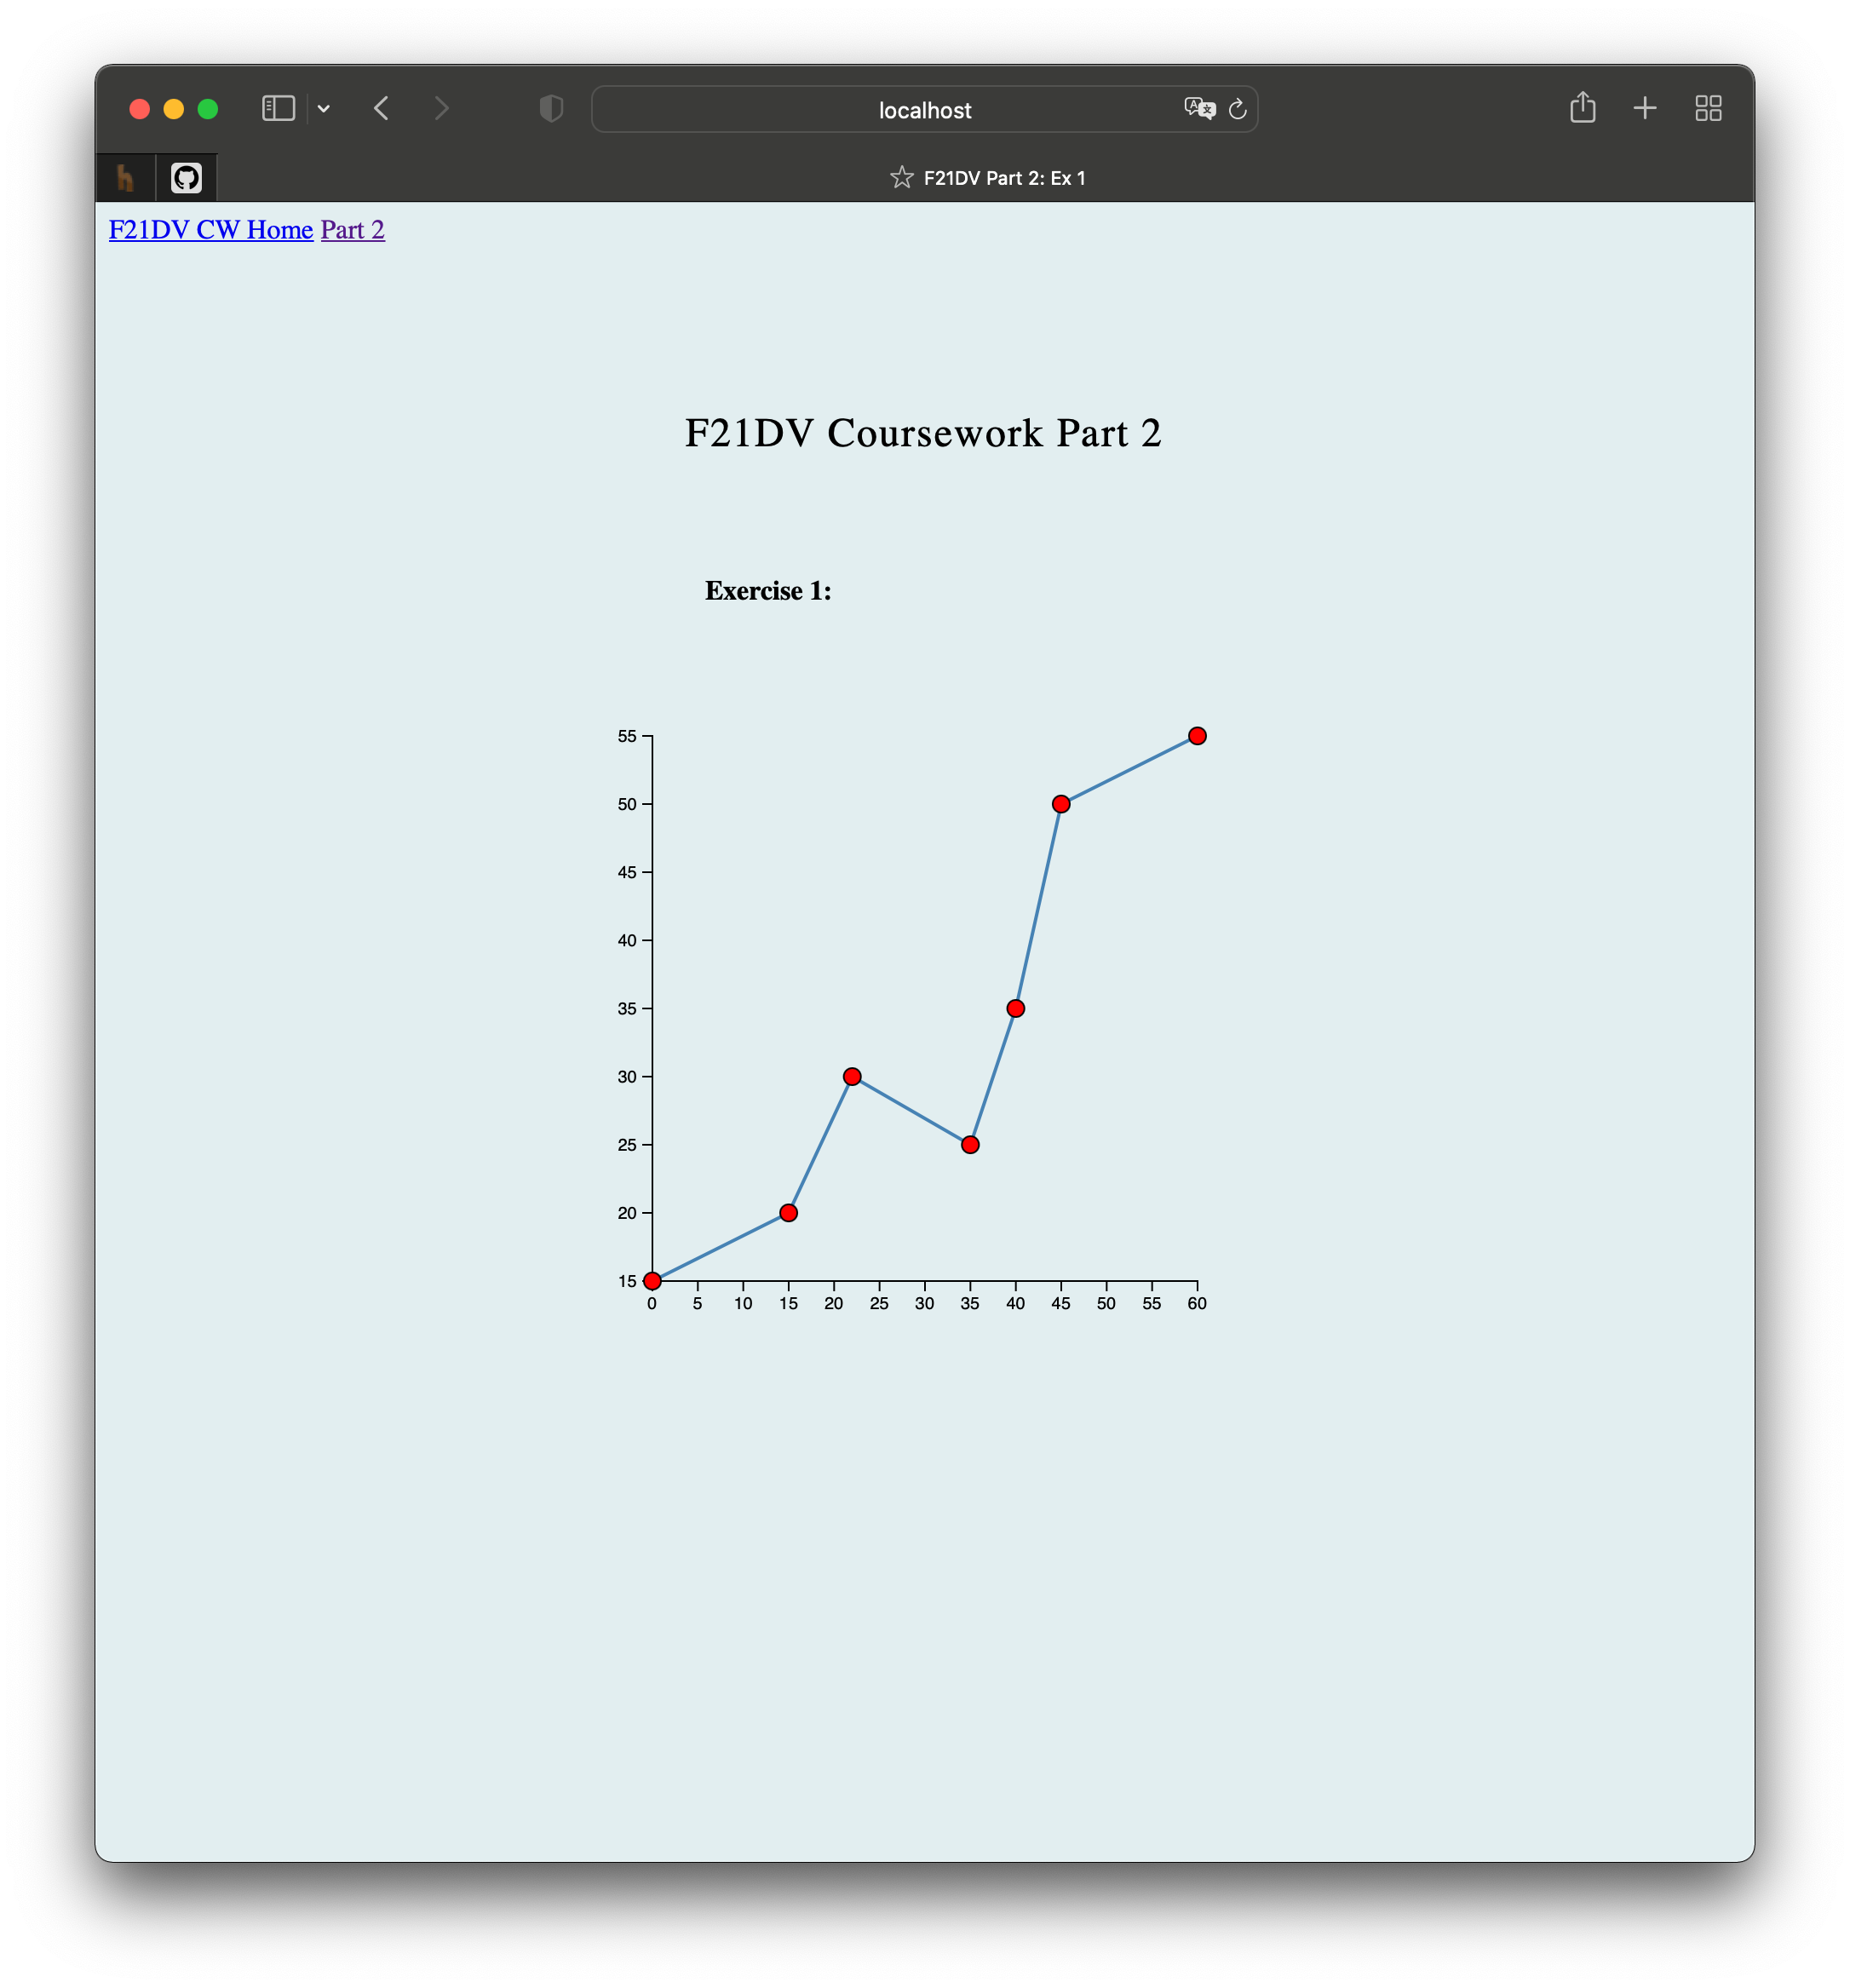
\includegraphics[width = 7.5cm]{images/ex1_1.png}
    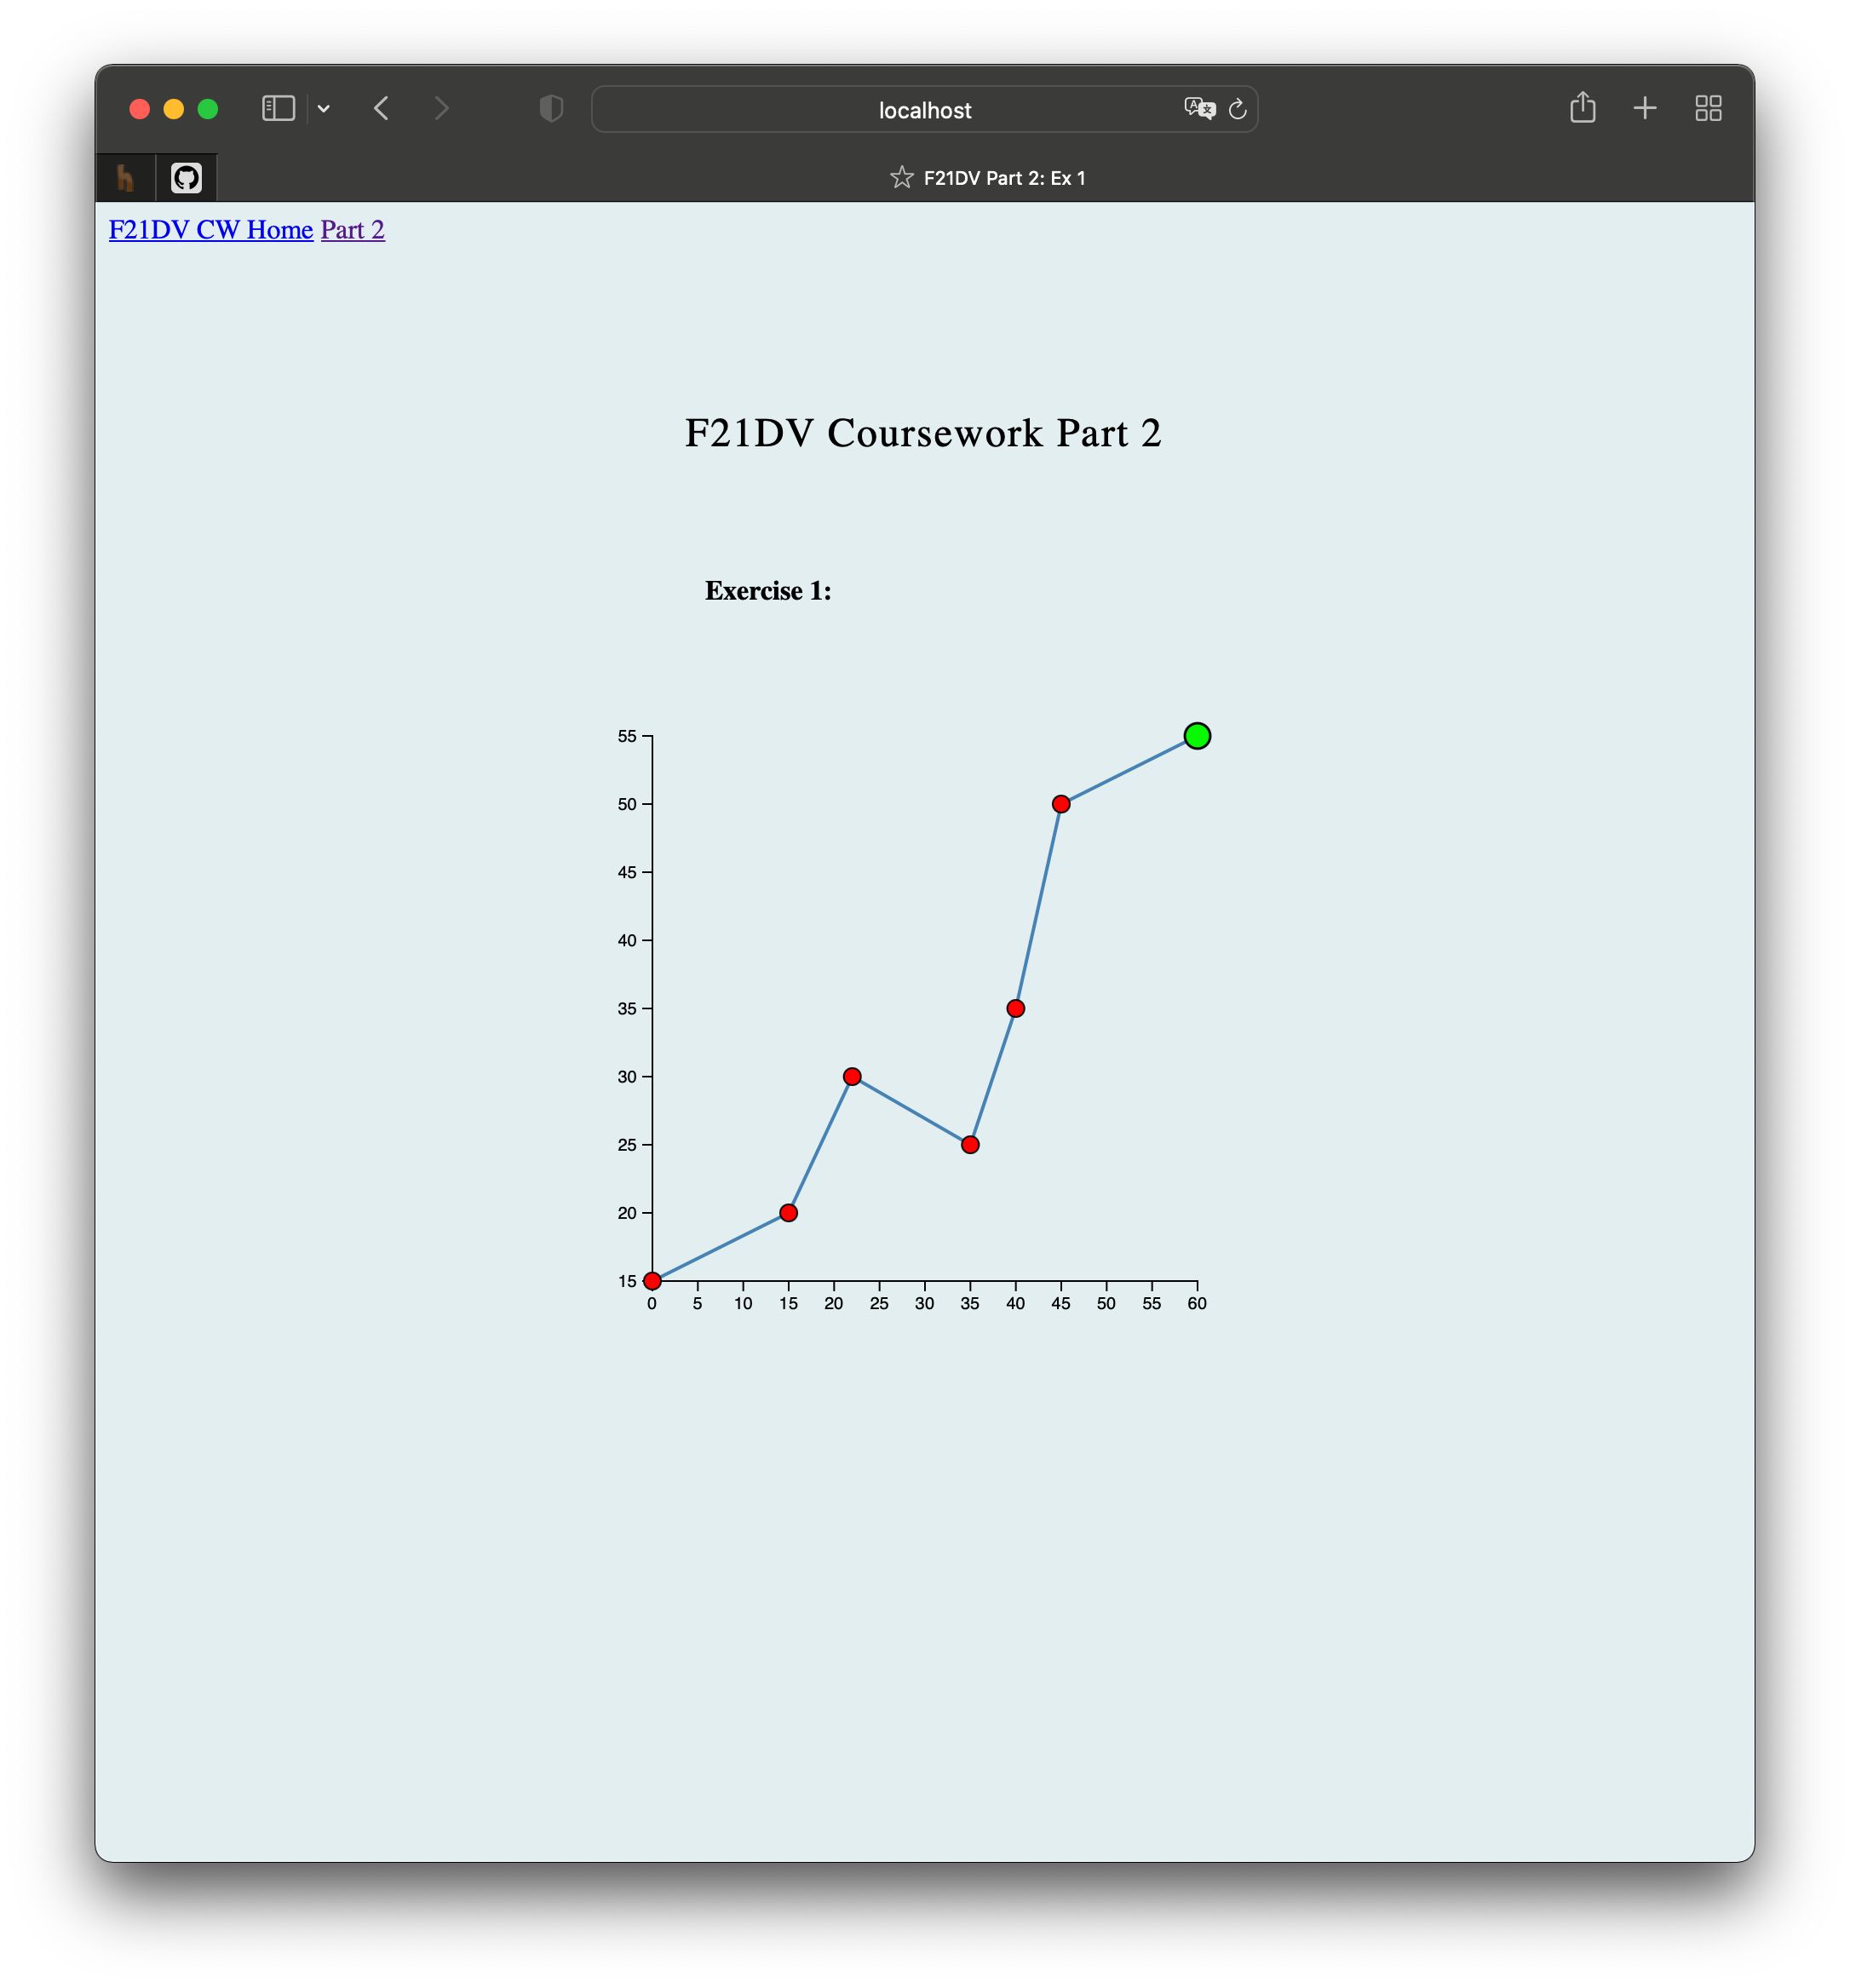
\includegraphics[width = 7.5cm]{images/ex1_2.png}
    \label{fig:ex1}
    \caption{Exercise 1}
\end{figure}
\FloatBarrier
Figure \ref{fig:ex1} shows a line chart with data points plotted on it. The right figure shows what happens when the mouse hovers upon a data point, the data point would pulse between red and green. *\textit{Can't seem to take a screenshot and capture the pointer}.

\newpage
\section{Exercise 2}
\begin{figure}[!ht]
    \centering
    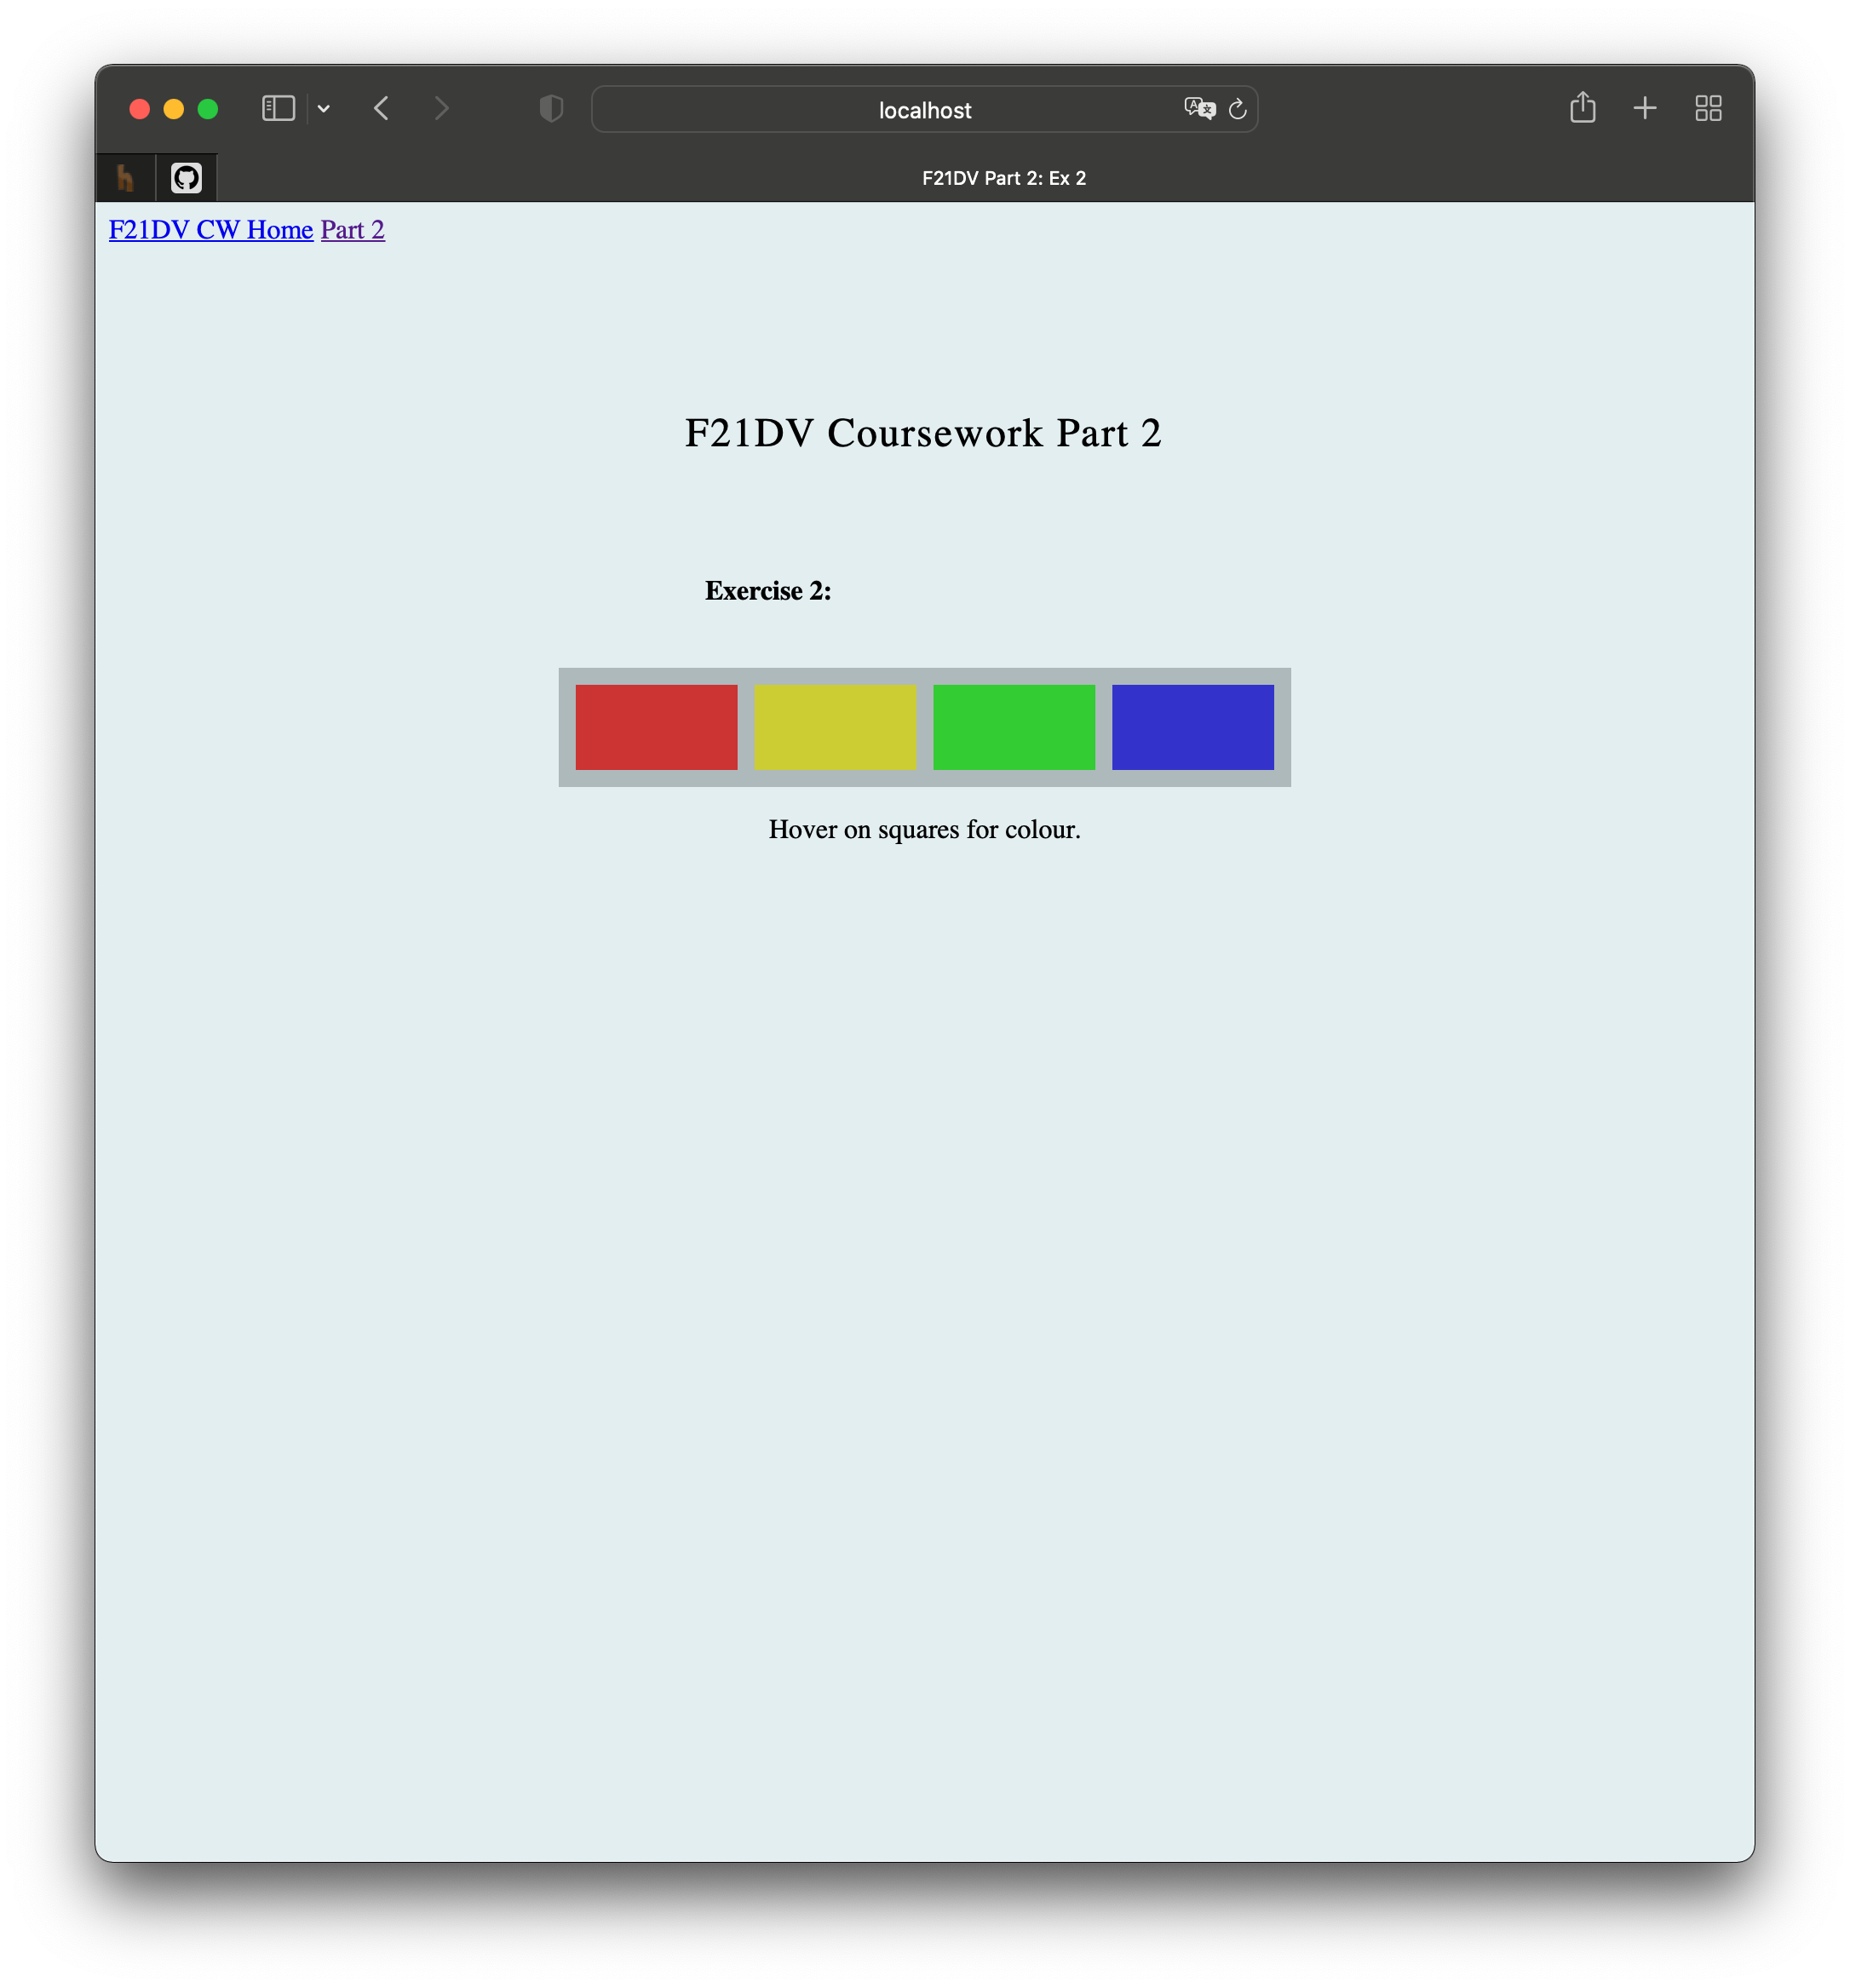
\includegraphics[width = 7.5cm]{images/ex2_1.png}
    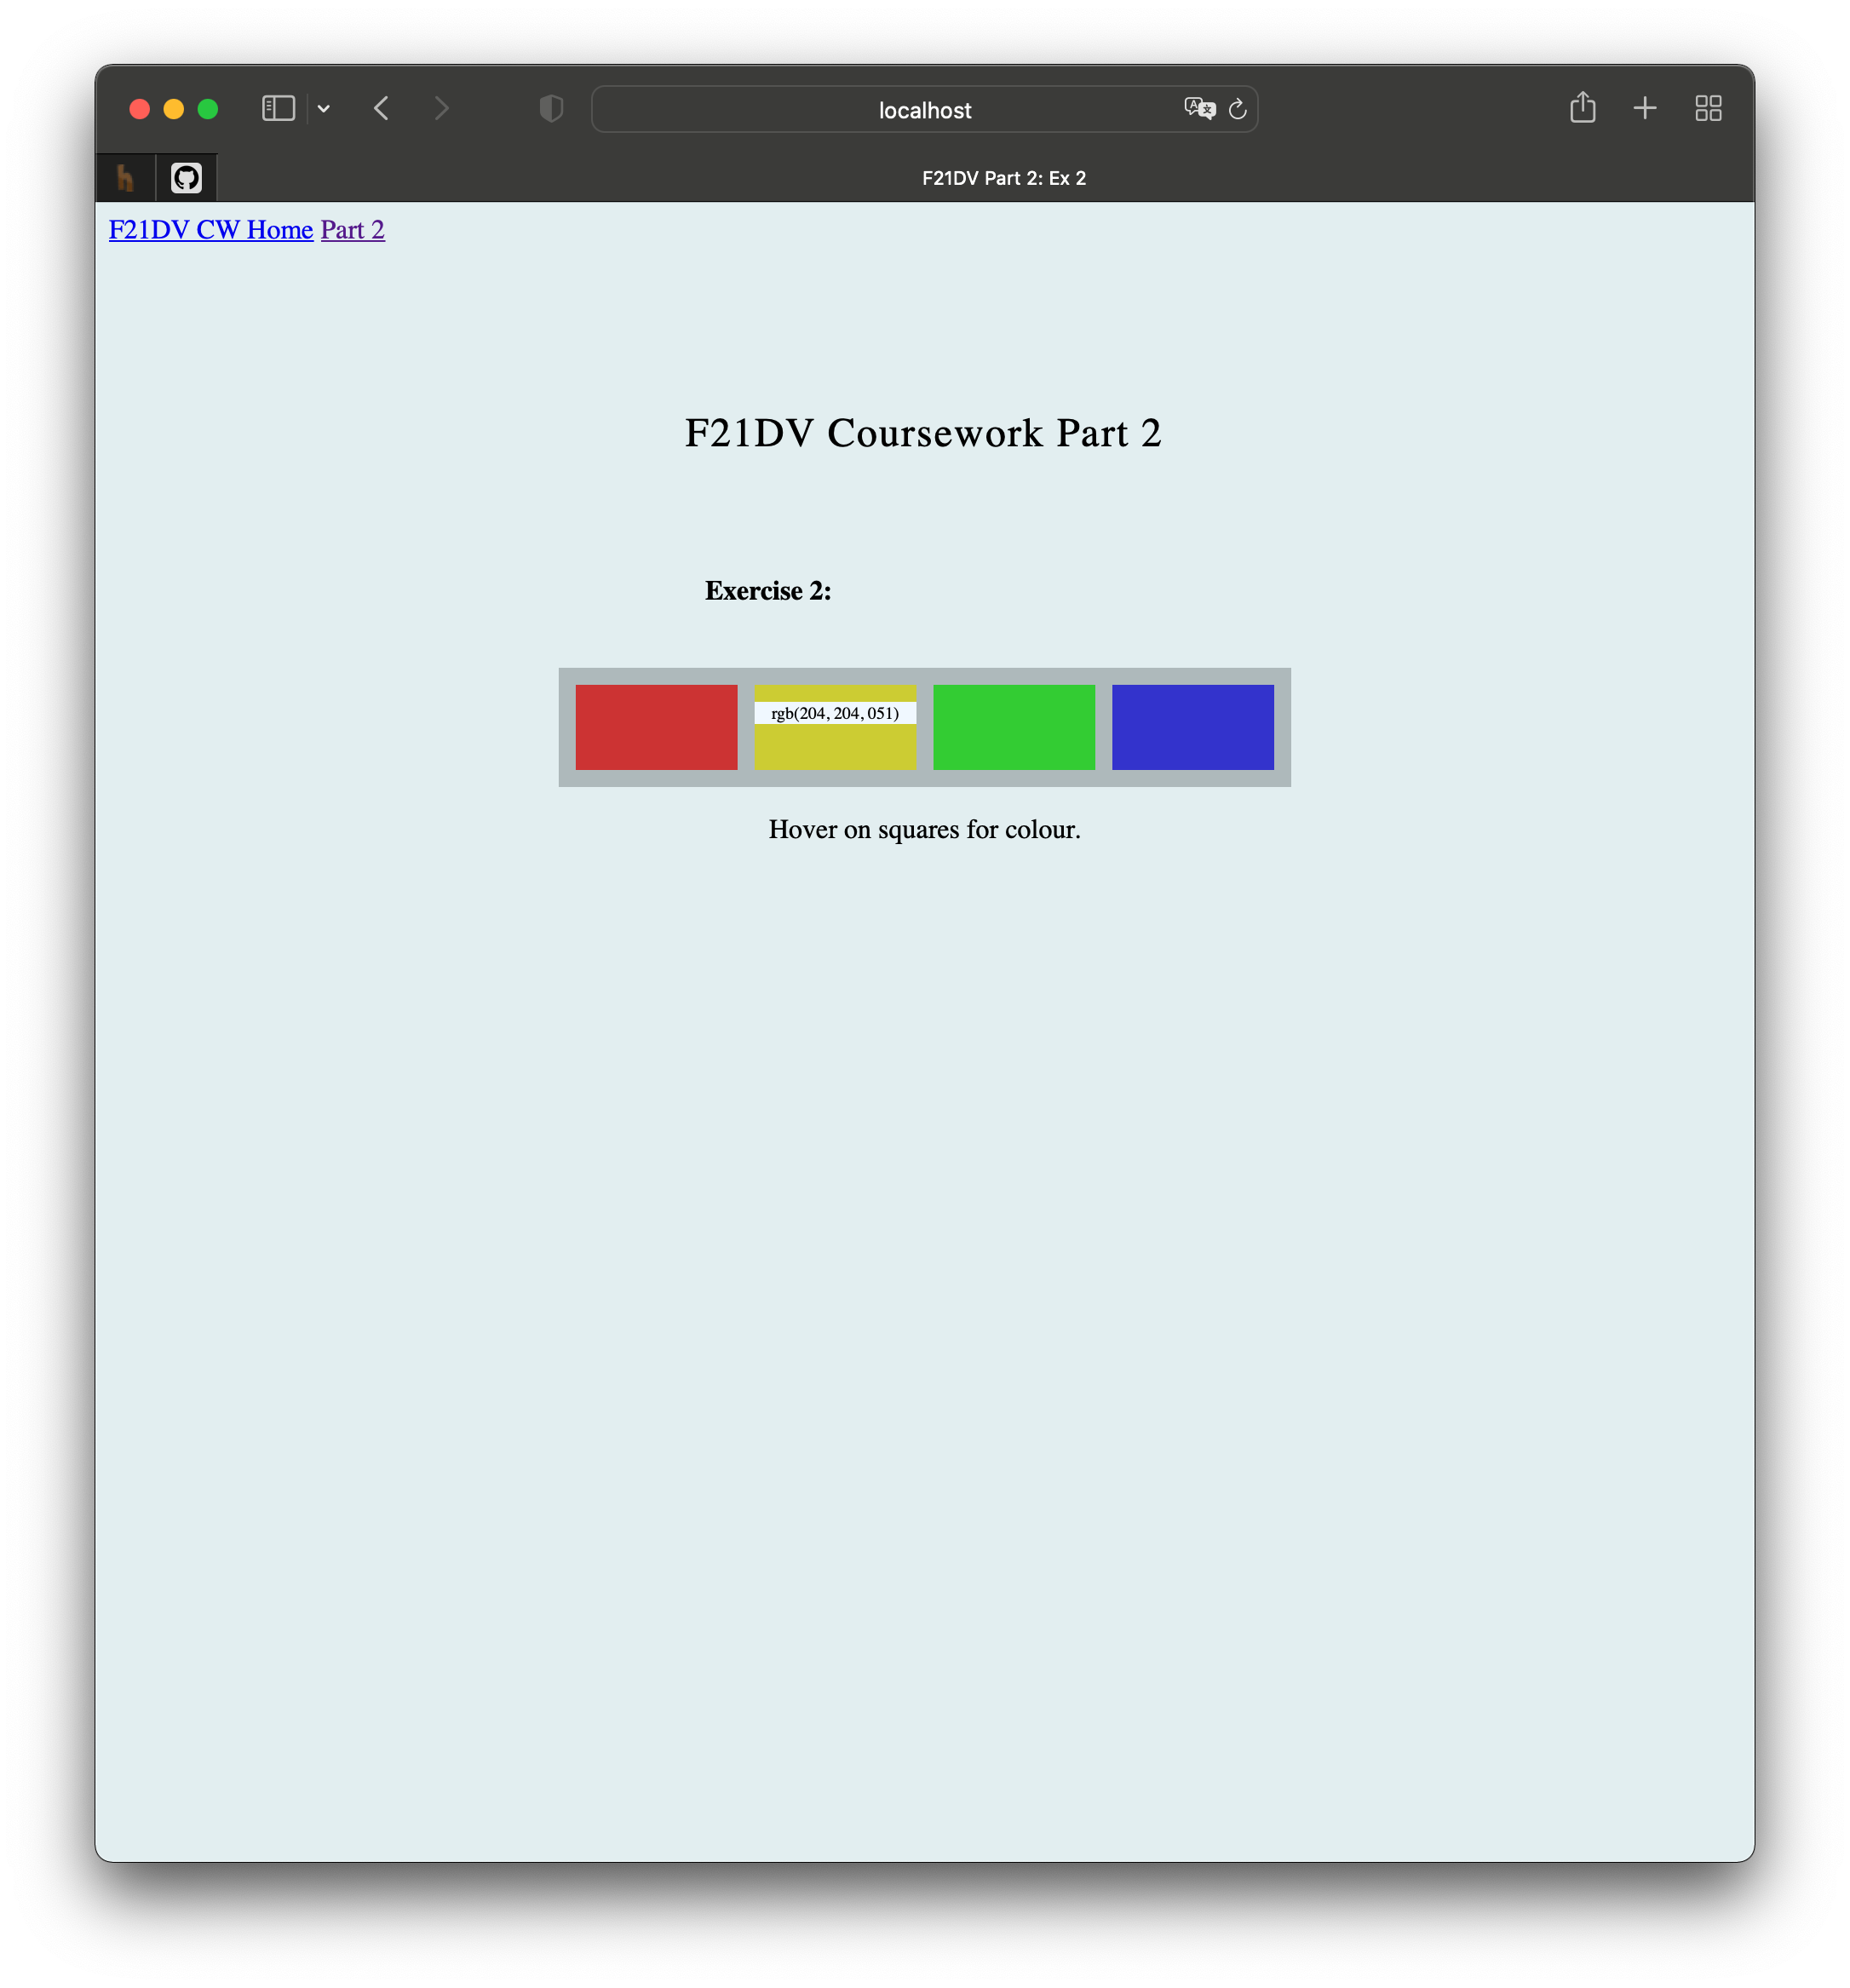
\includegraphics[width = 7.5cm]{images/ex2_2.png}
    \label{fig:ex2}
    \caption{Exercise 2}
\end{figure}
\FloatBarrier
% \lstinputlisting[language=JavaScript]{../../public/js/part2/task2.js}
Figure \ref{fig:ex2} shows 4 blocks with different colours. The blocks are just a div defined within a grid. Each block also has a fill colour defined using the \verb|Rgb()| colour method, as shown in line 10. Upon hovering the mouse on the div, the div would show a text element displaying the Rgb colour. This effect is done using the css \verb|:hover| method.

\newpage
\section{Exercise 3}
\begin{figure}[!ht]
    \centering
    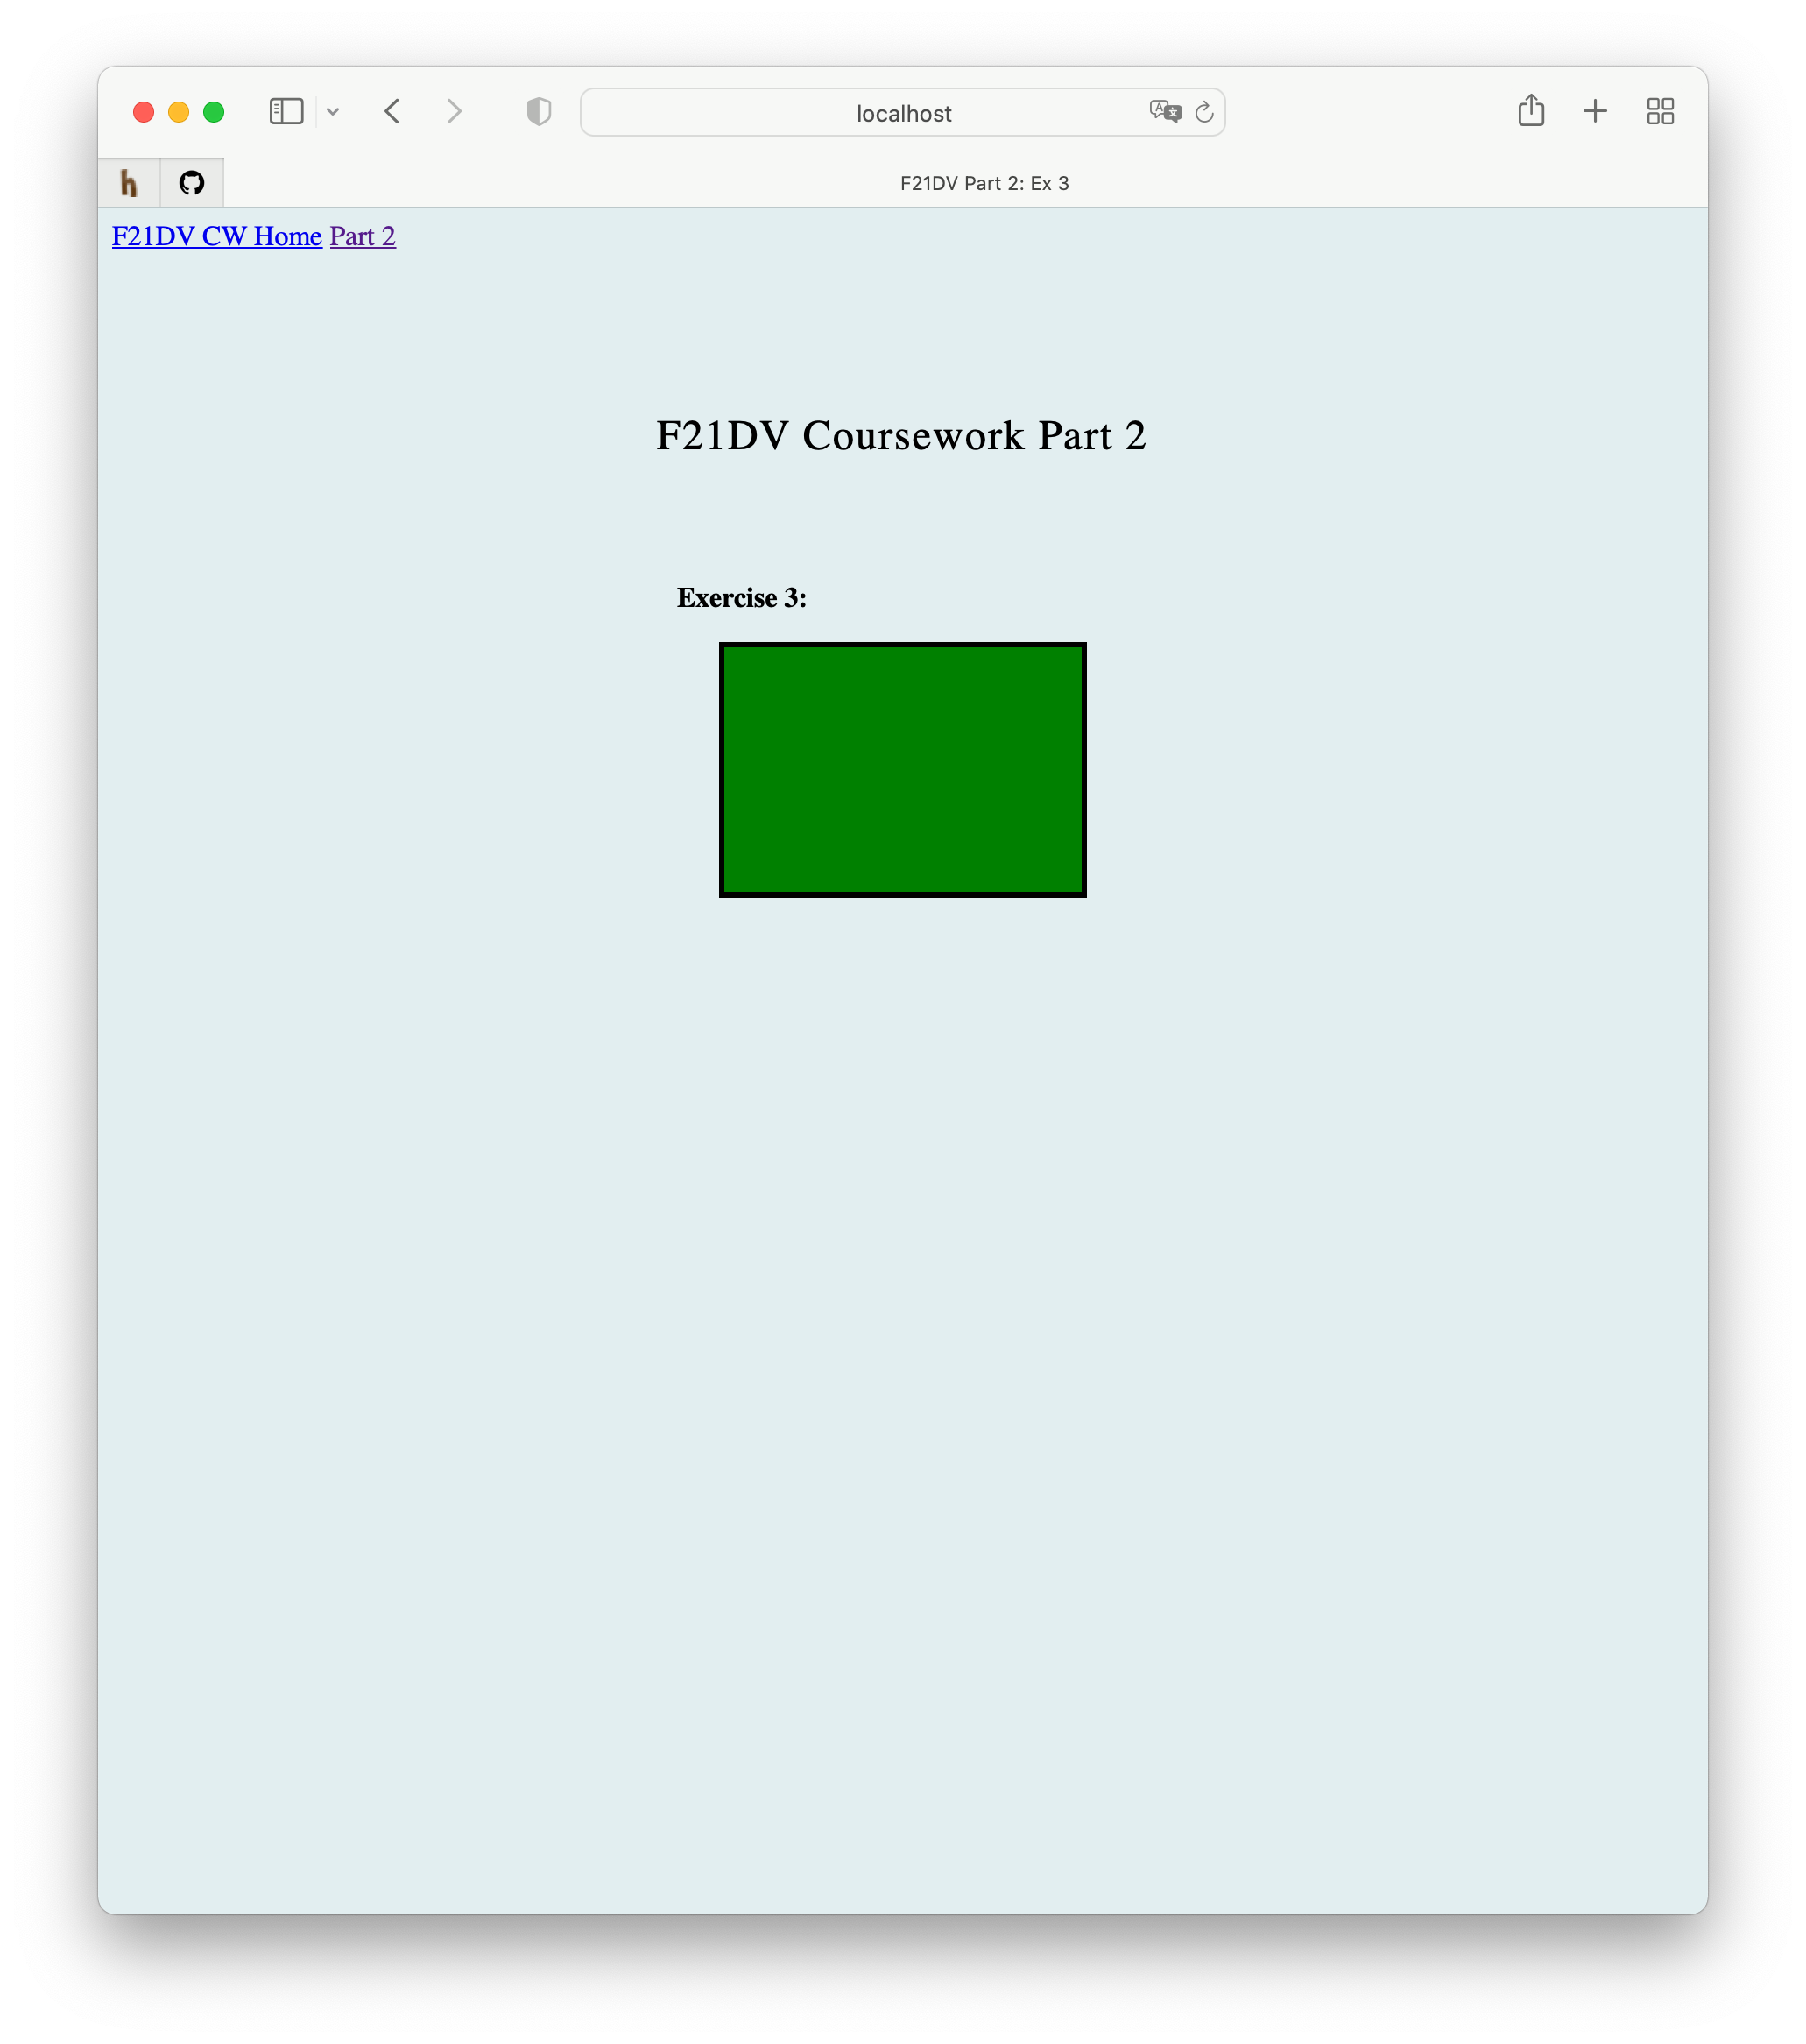
\includegraphics[width = 7.5cm]{images/ex3_1.png}
    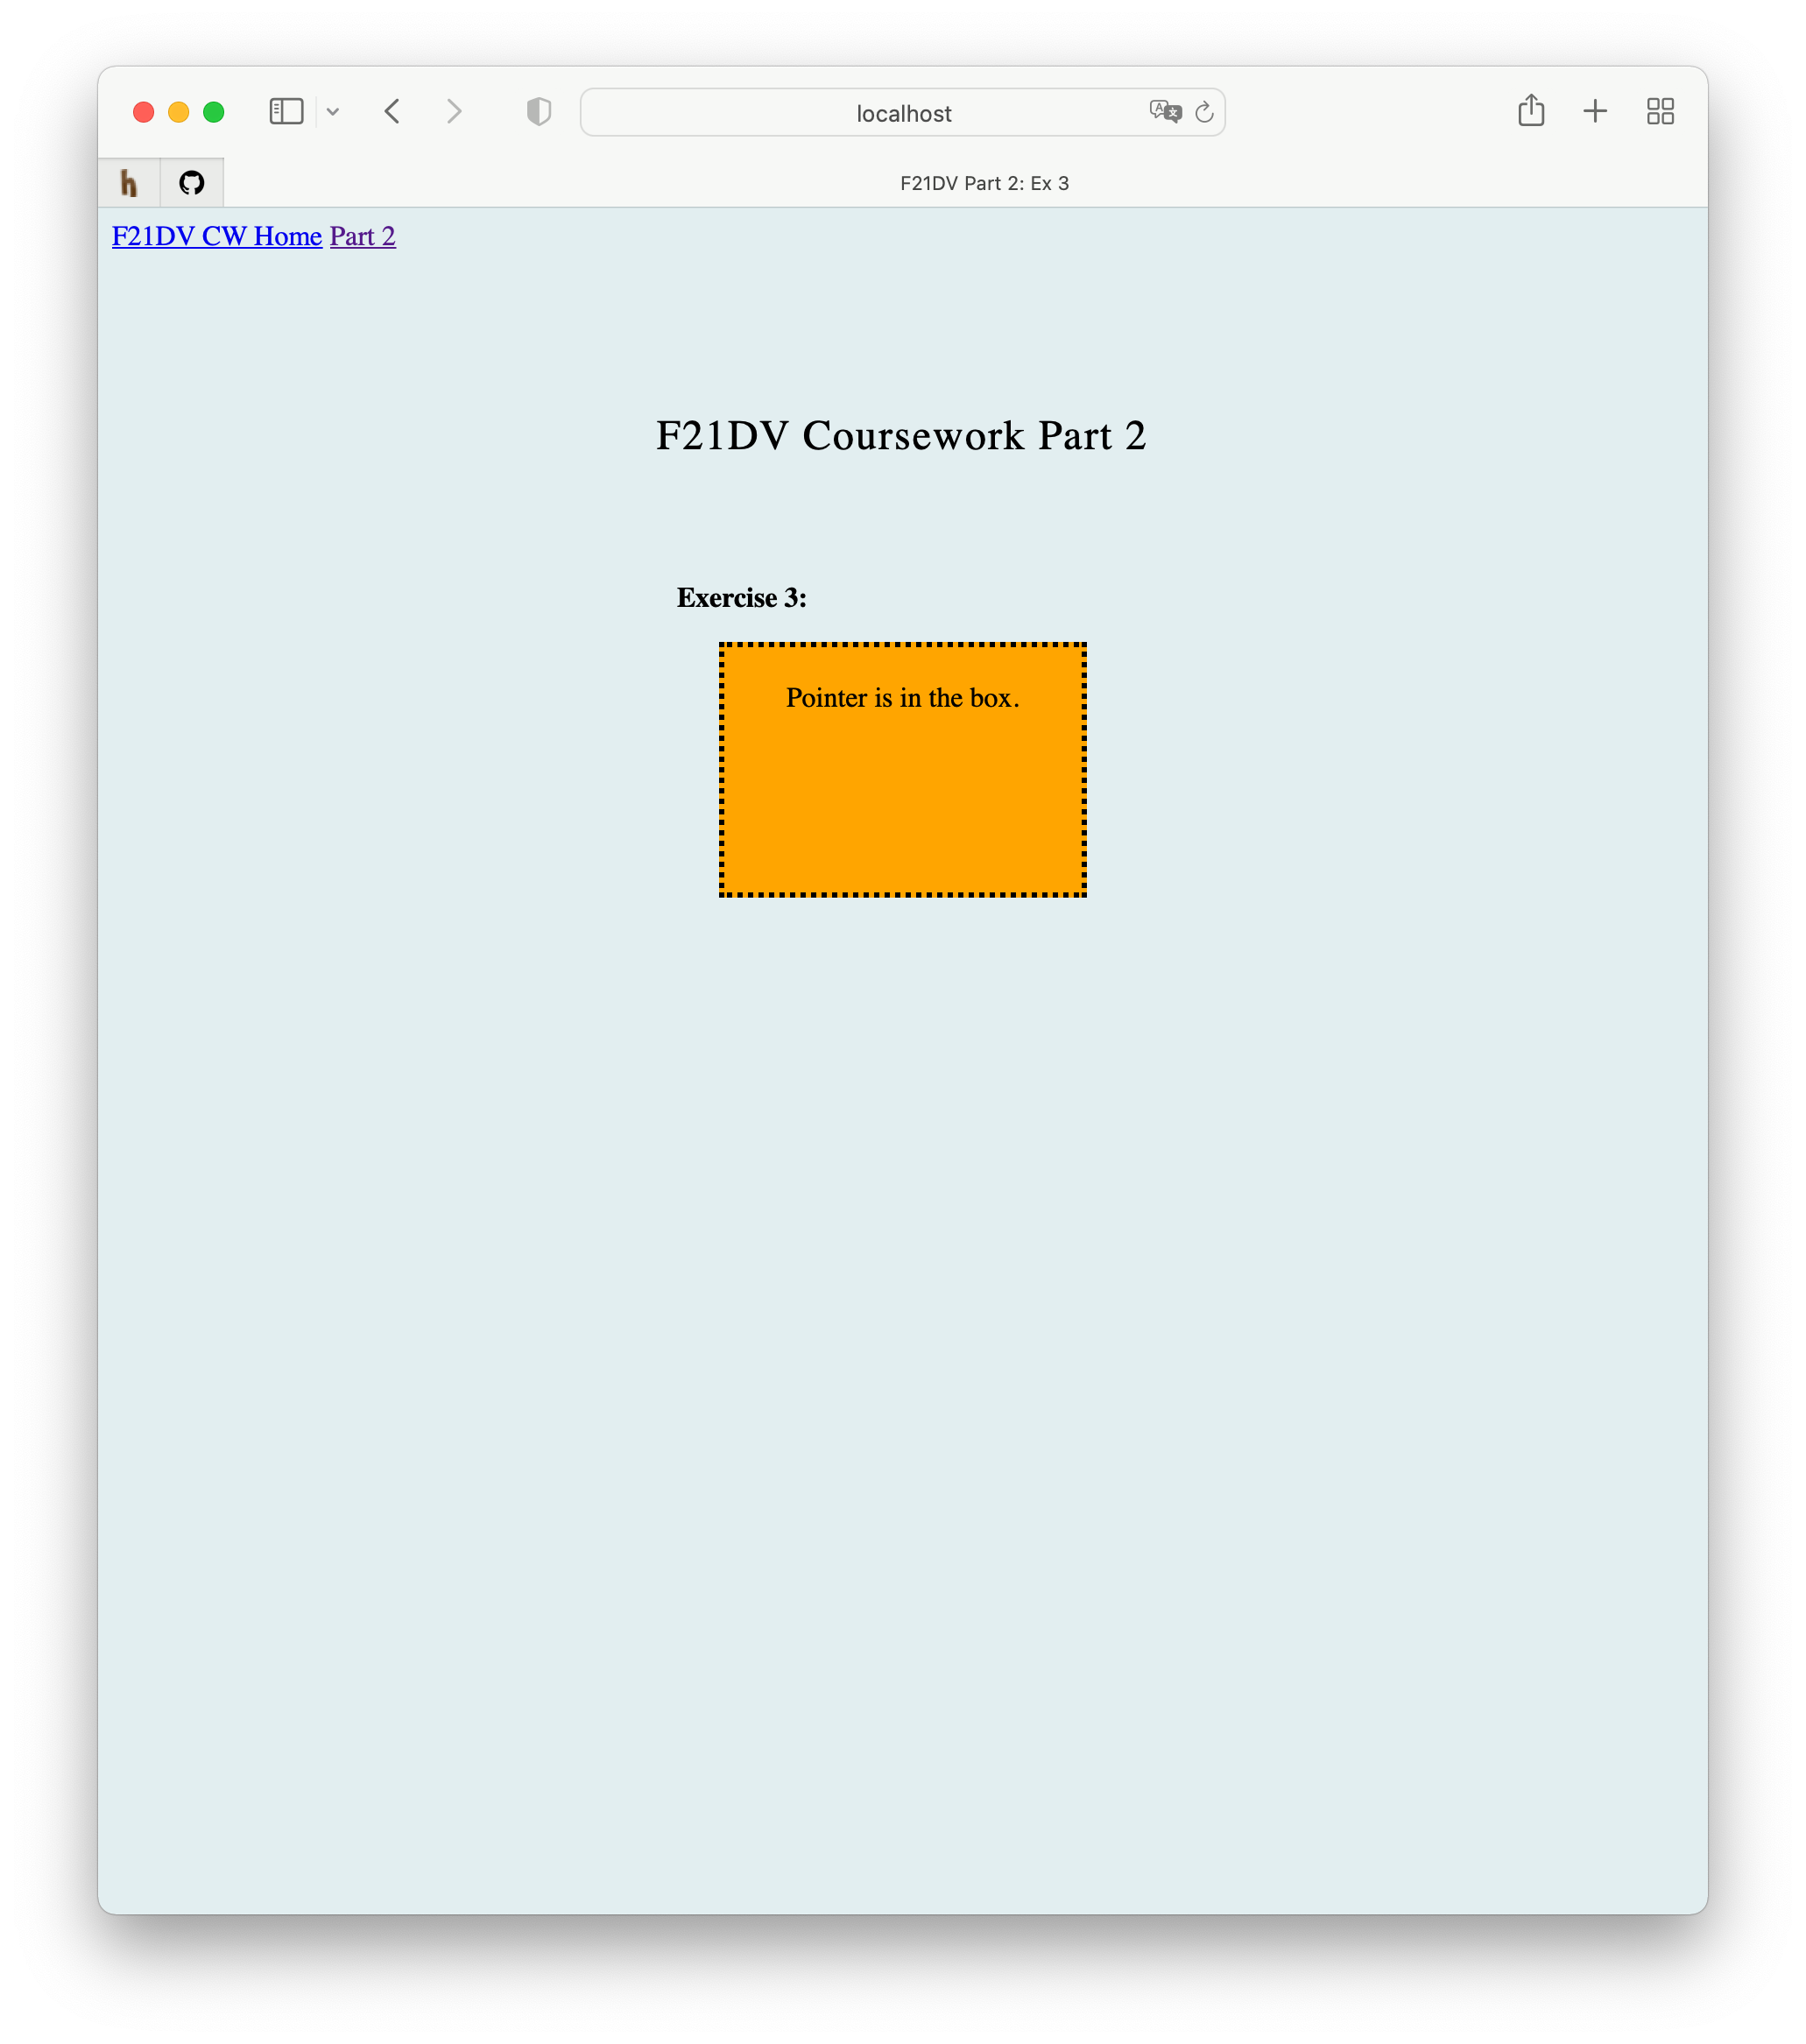
\includegraphics[width = 7.5cm]{images/ex3_2.png}
    \label{fig:ex3}
    \caption{Exercise 3}
\end{figure}
\FloatBarrier
\lstinputlisting[language=JavaScript]{../../public/js/part2/task3.js}
Figure \ref{fig:ex3} shows a block thats green colour. Upon mouse hover on the box, the box now shows a text that says `Pointer is in the box', its colour is now orange, and it has a new type of border. This is done using the \verb|.on()| function.

\newpage
\section{Exercise 4}
\begin{figure}[!ht]
    \centering
    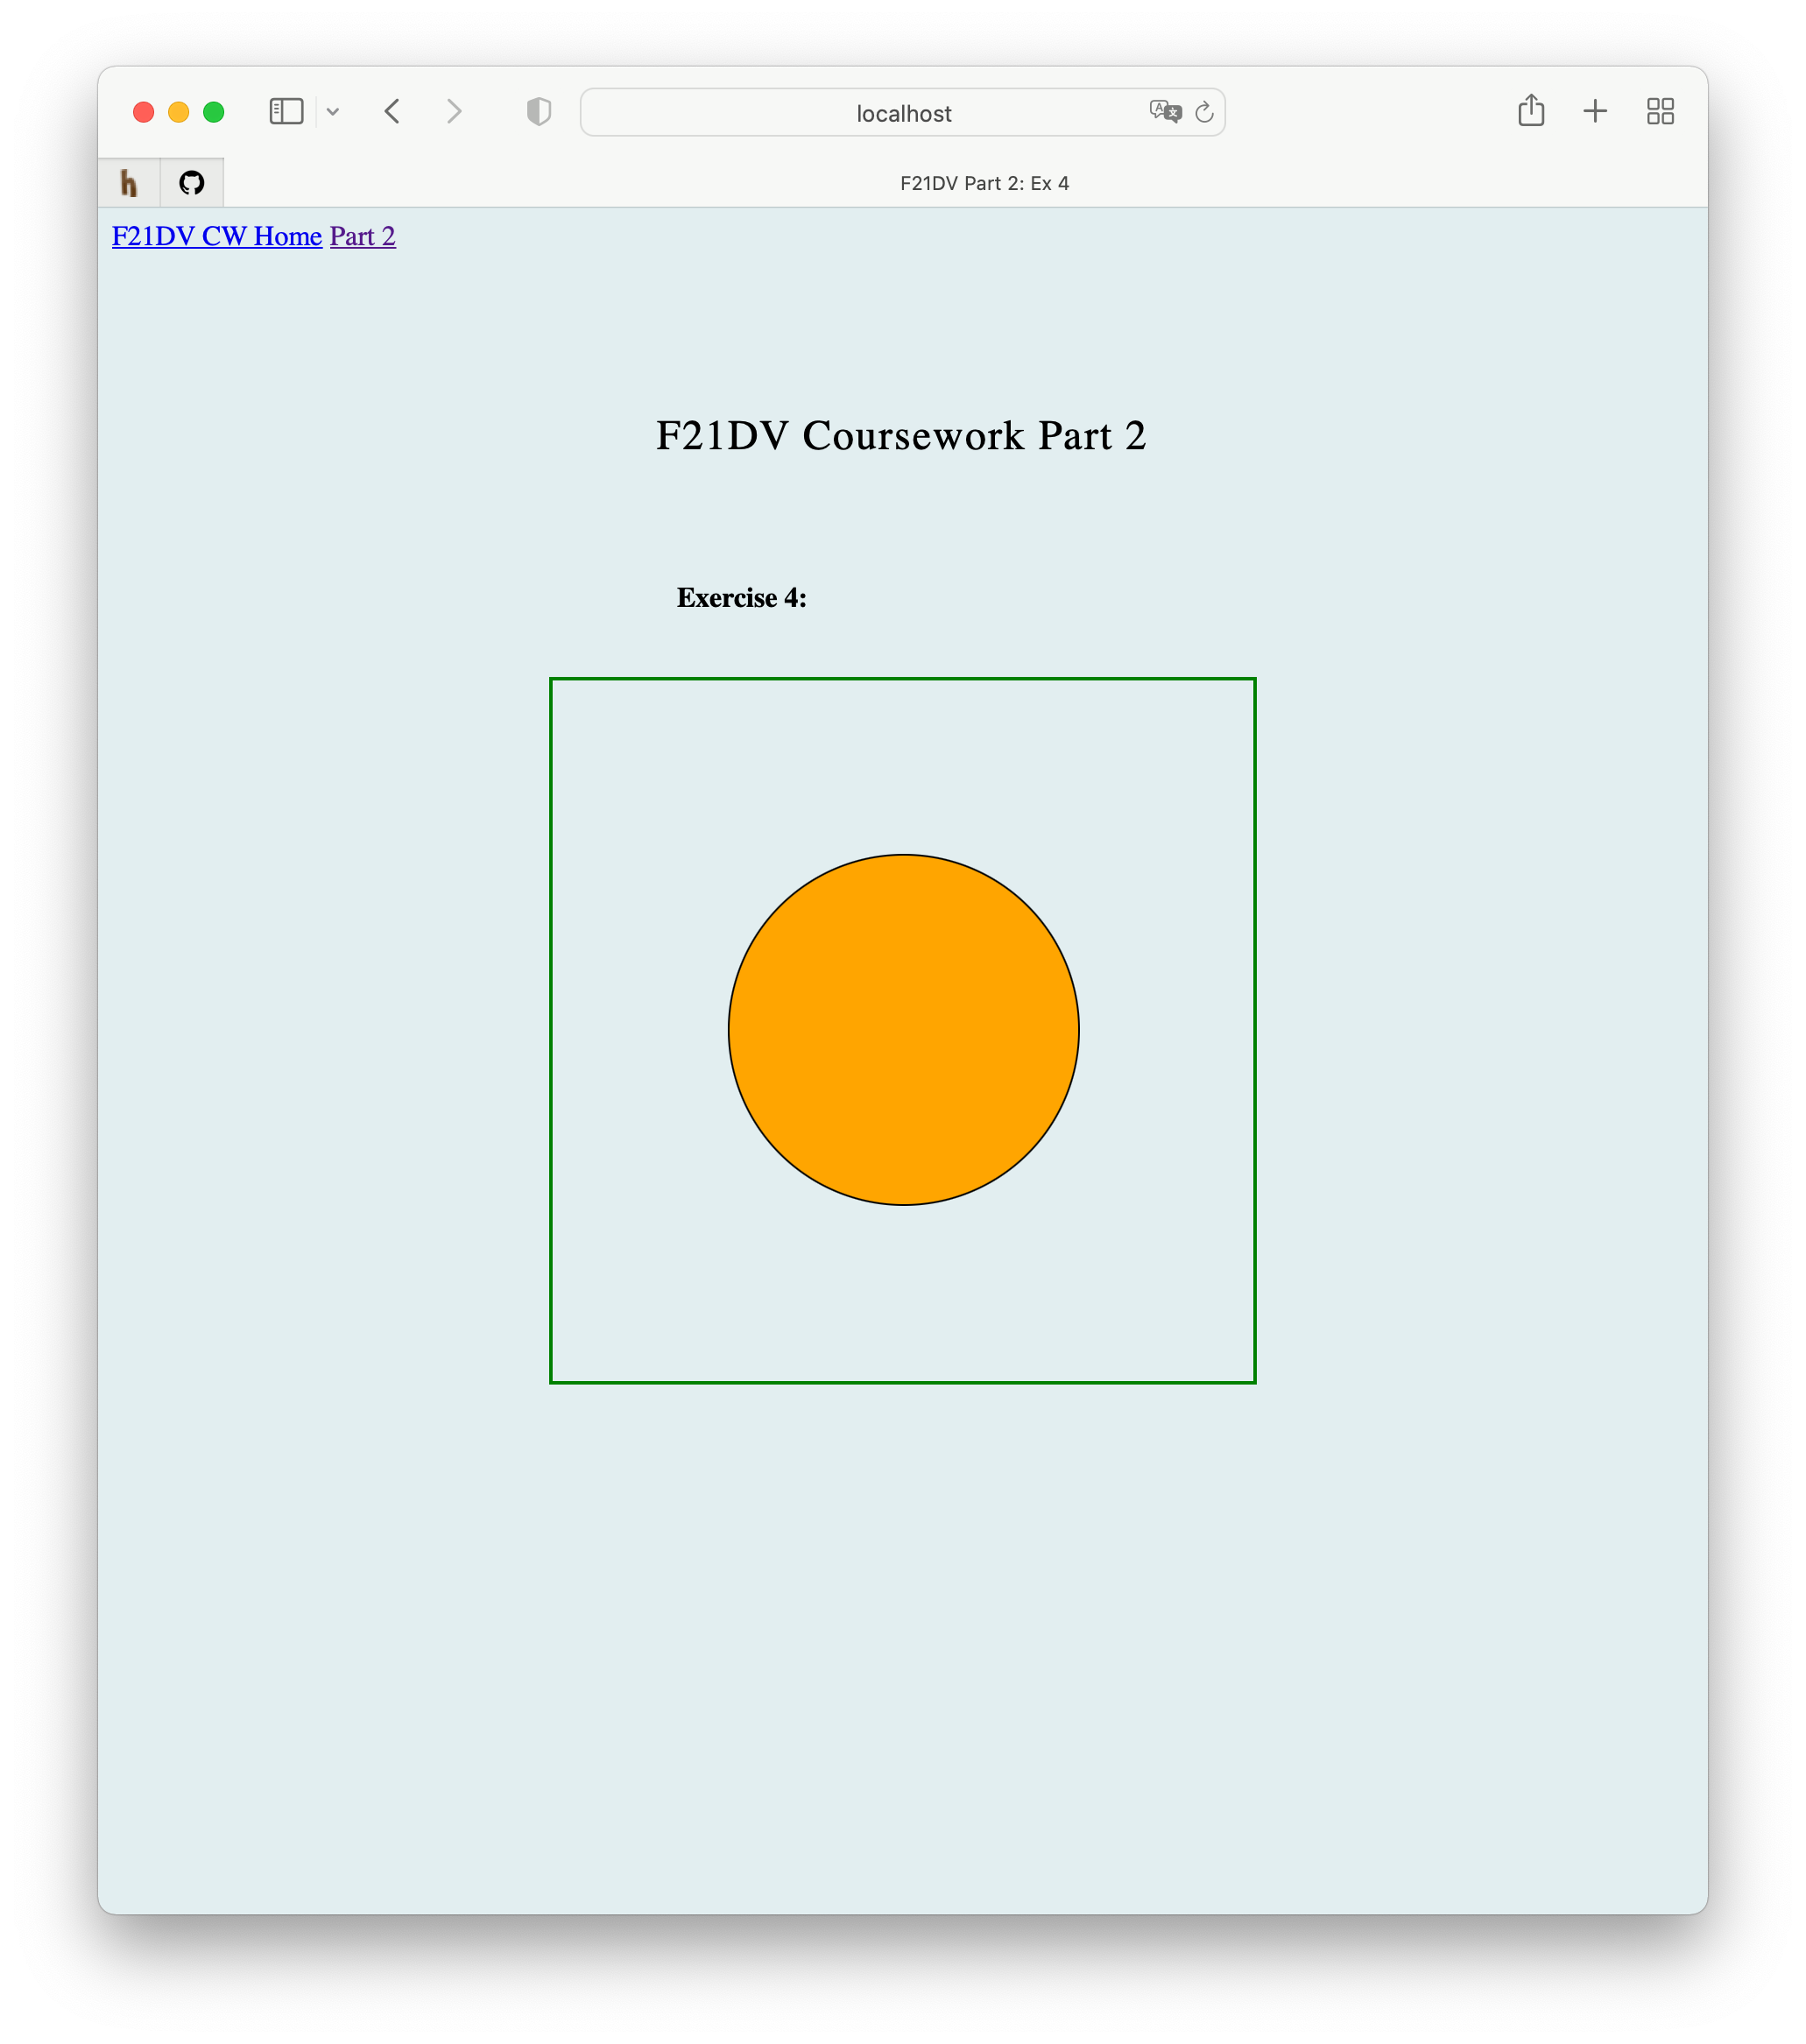
\includegraphics[width = 7.5cm]{images/ex4_1.png}
    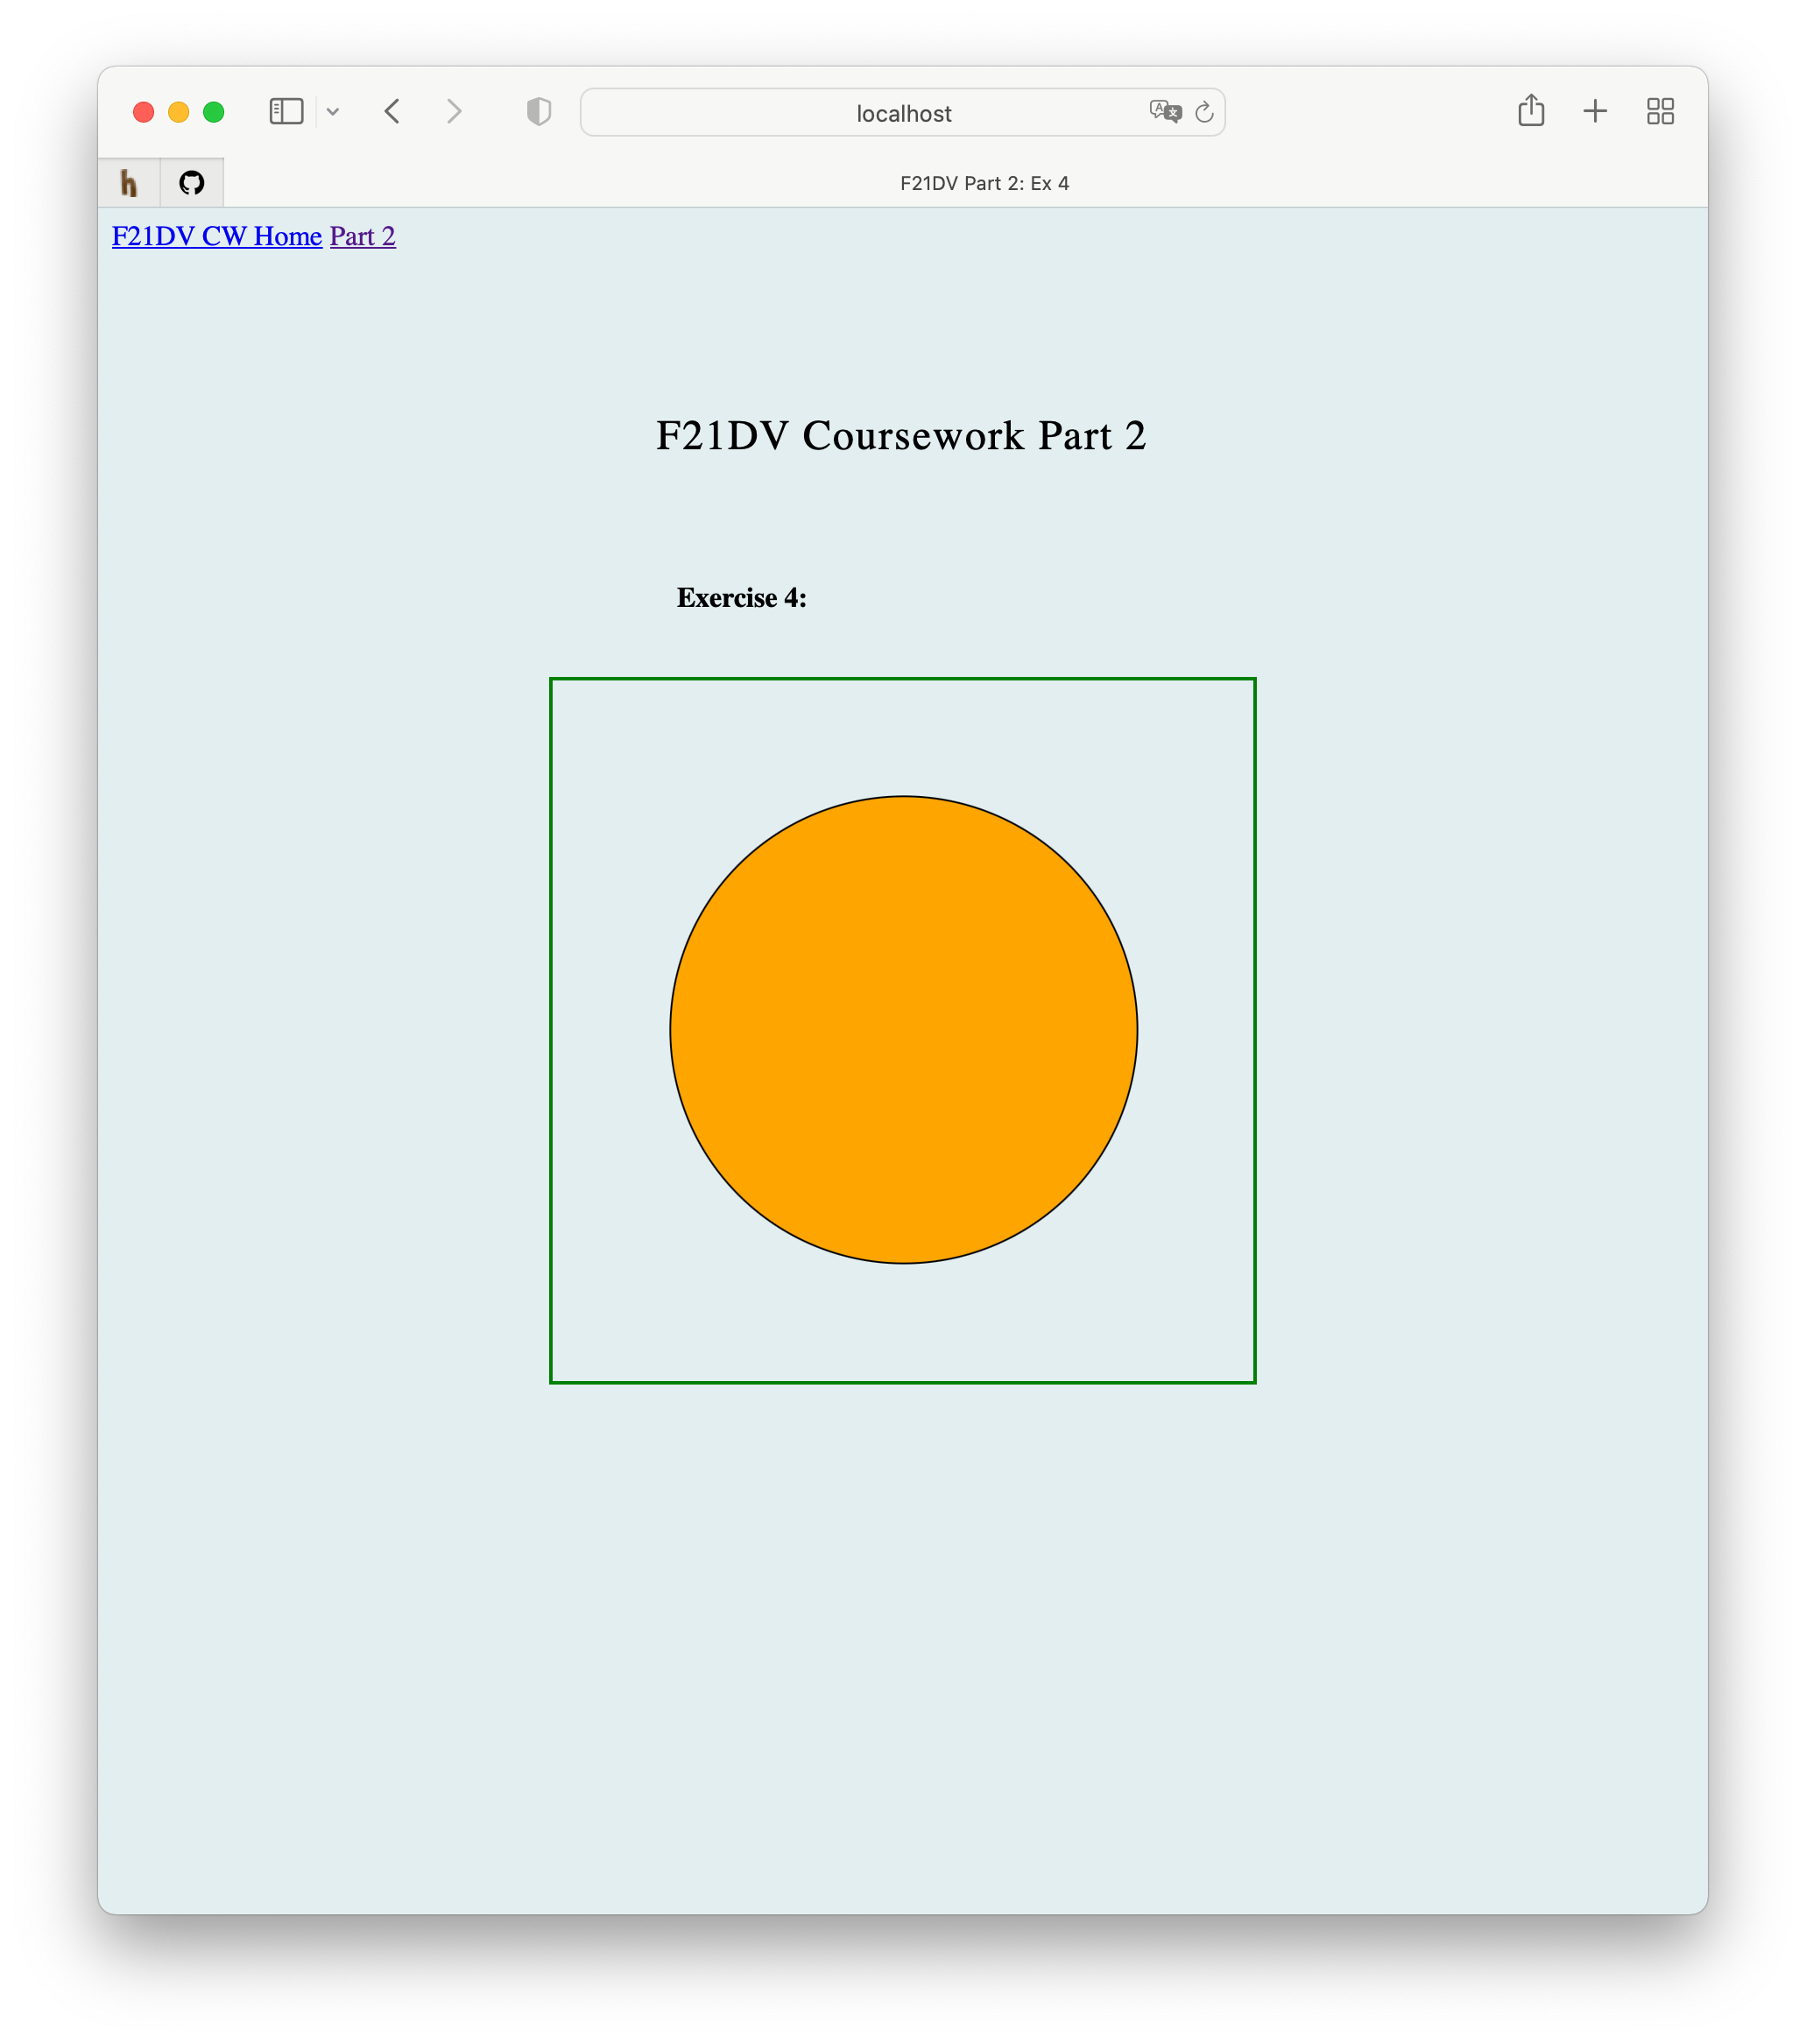
\includegraphics[width = 7.5cm]{images/ex4_2.png}
    \label{fig:ex4}
    \caption{Exercise 4}
\end{figure}
\FloatBarrier
% \lstinputlisting[language=JavaScript]{../../public/js/part2/task4.js}
Figure \ref{fig:ex4} shows an SVG object with a circle in the middle. Upon hovering on the circle, the circle enlarges. This time, the action was modeled using d3 transitions instead of css :hover method. I've added transtitions upon mouse hover and out.

\newpage
\section{Exercise 5}
\begin{figure}[!ht]
    \centering
    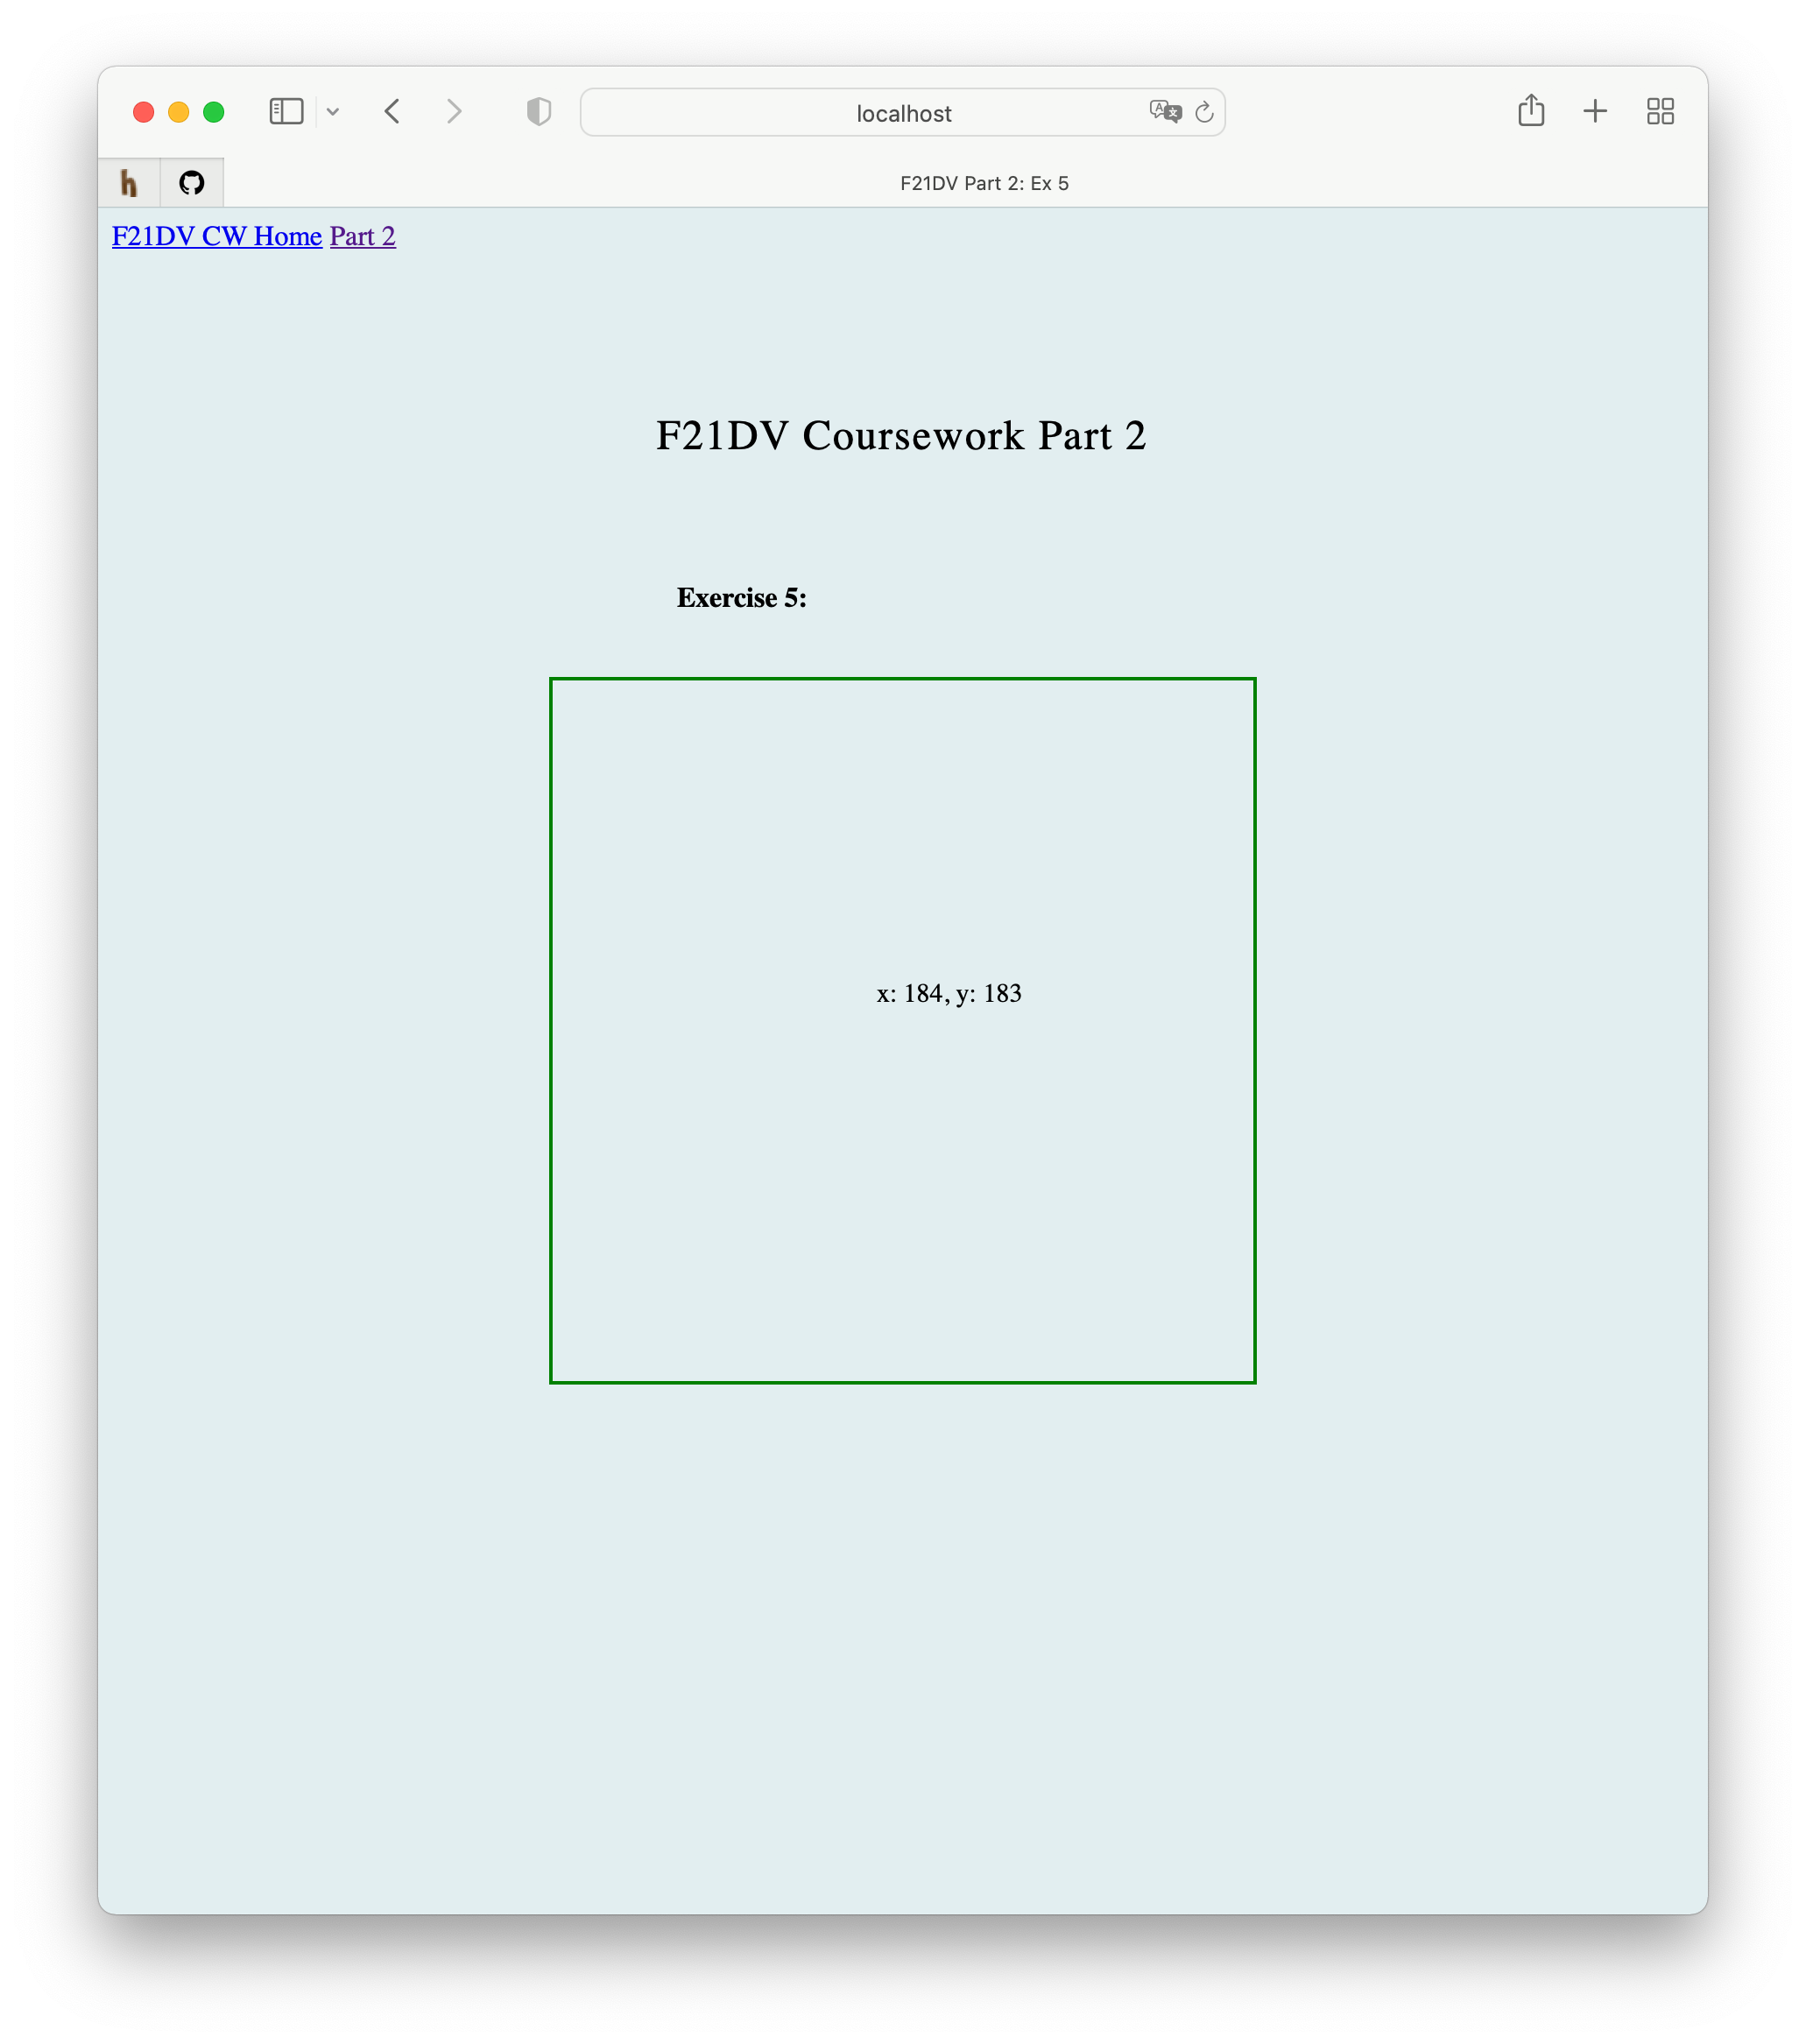
\includegraphics[width = 7.5cm]{images/ex5.png}
    % 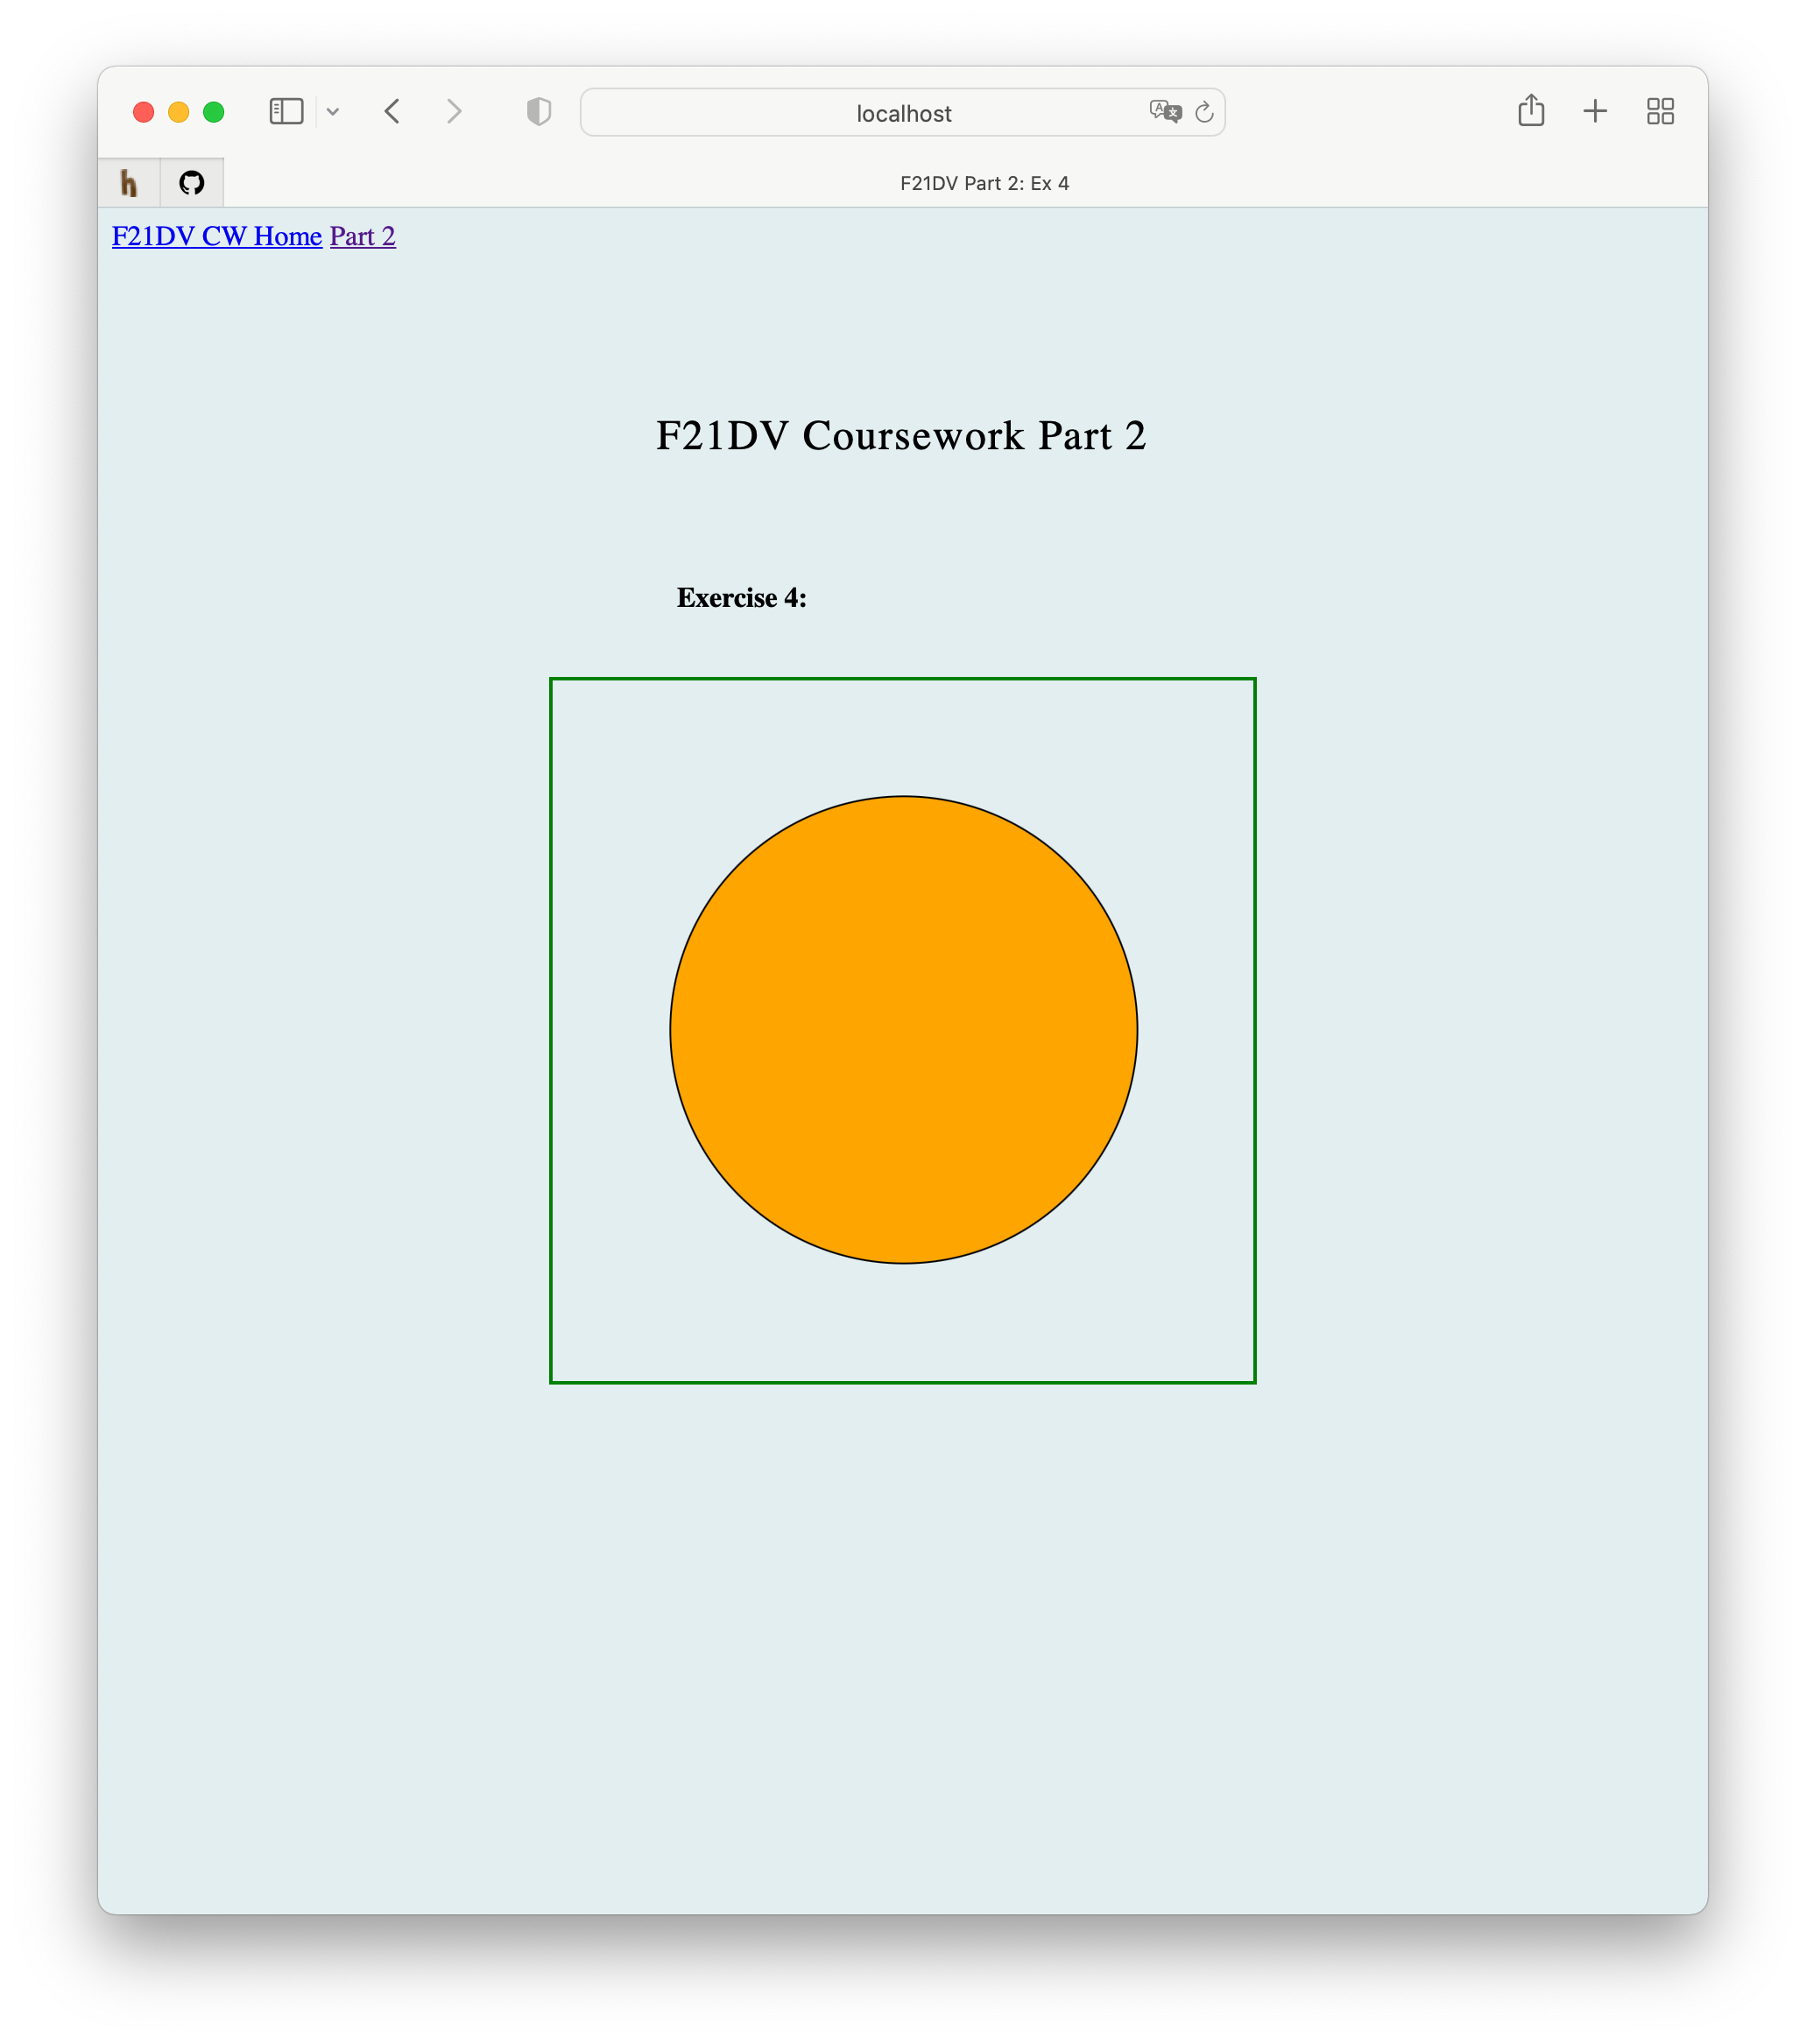
\includegraphics[width = 7.5cm]{images/ex4_2.png}
    \label{fig:ex5}
    \caption{Exercise 5}
\end{figure}
\FloatBarrier
% \lstinputlisting[language=JavaScript]{../../public/js/part2/task5.js}
Figure \ref{fig:ex5} shows an emptey svg object, and upon mouse hover, it would show the corredinated of the mouse. There was also a pre-appended empty text box. To show the x-y coordinates, this is done using the event data of the mouse movement. Then using the data, I modified the `x' and `y' attribute of the text box.

\newpage
\section{Exercise 6}
\begin{figure}[!ht]
    \centering
    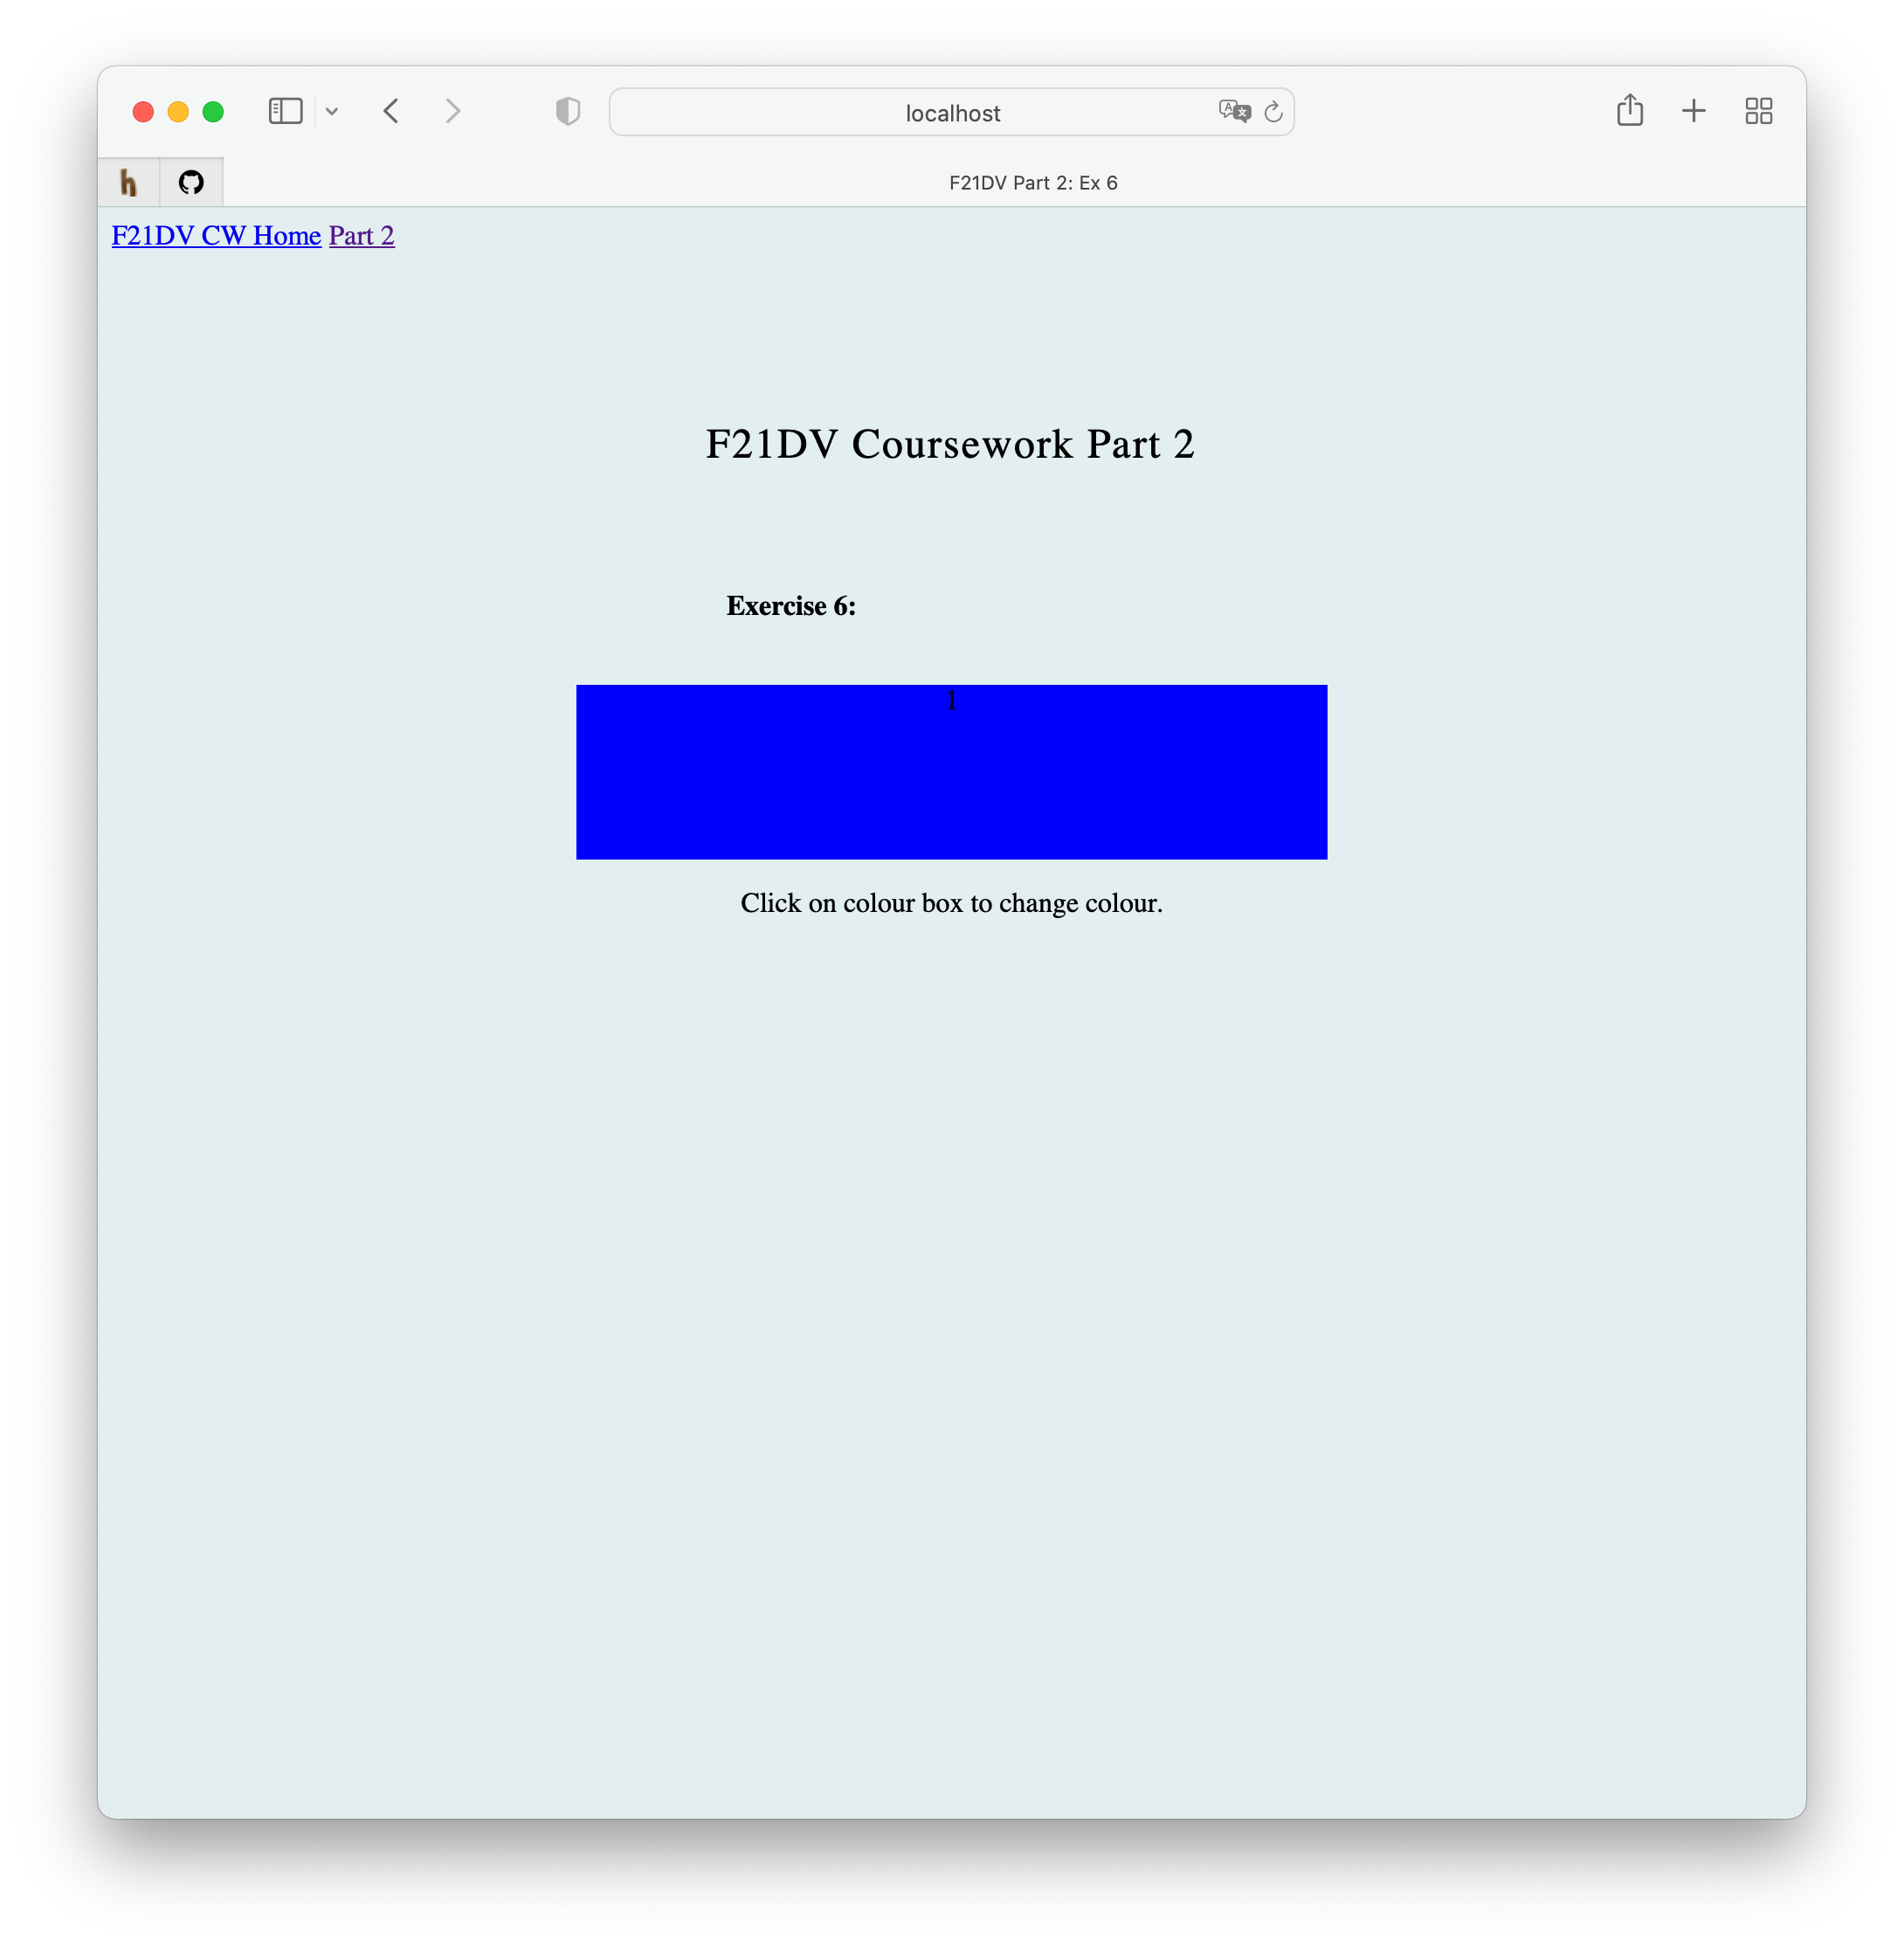
\includegraphics[width = 7.5cm]{images/ex6_1.png}
    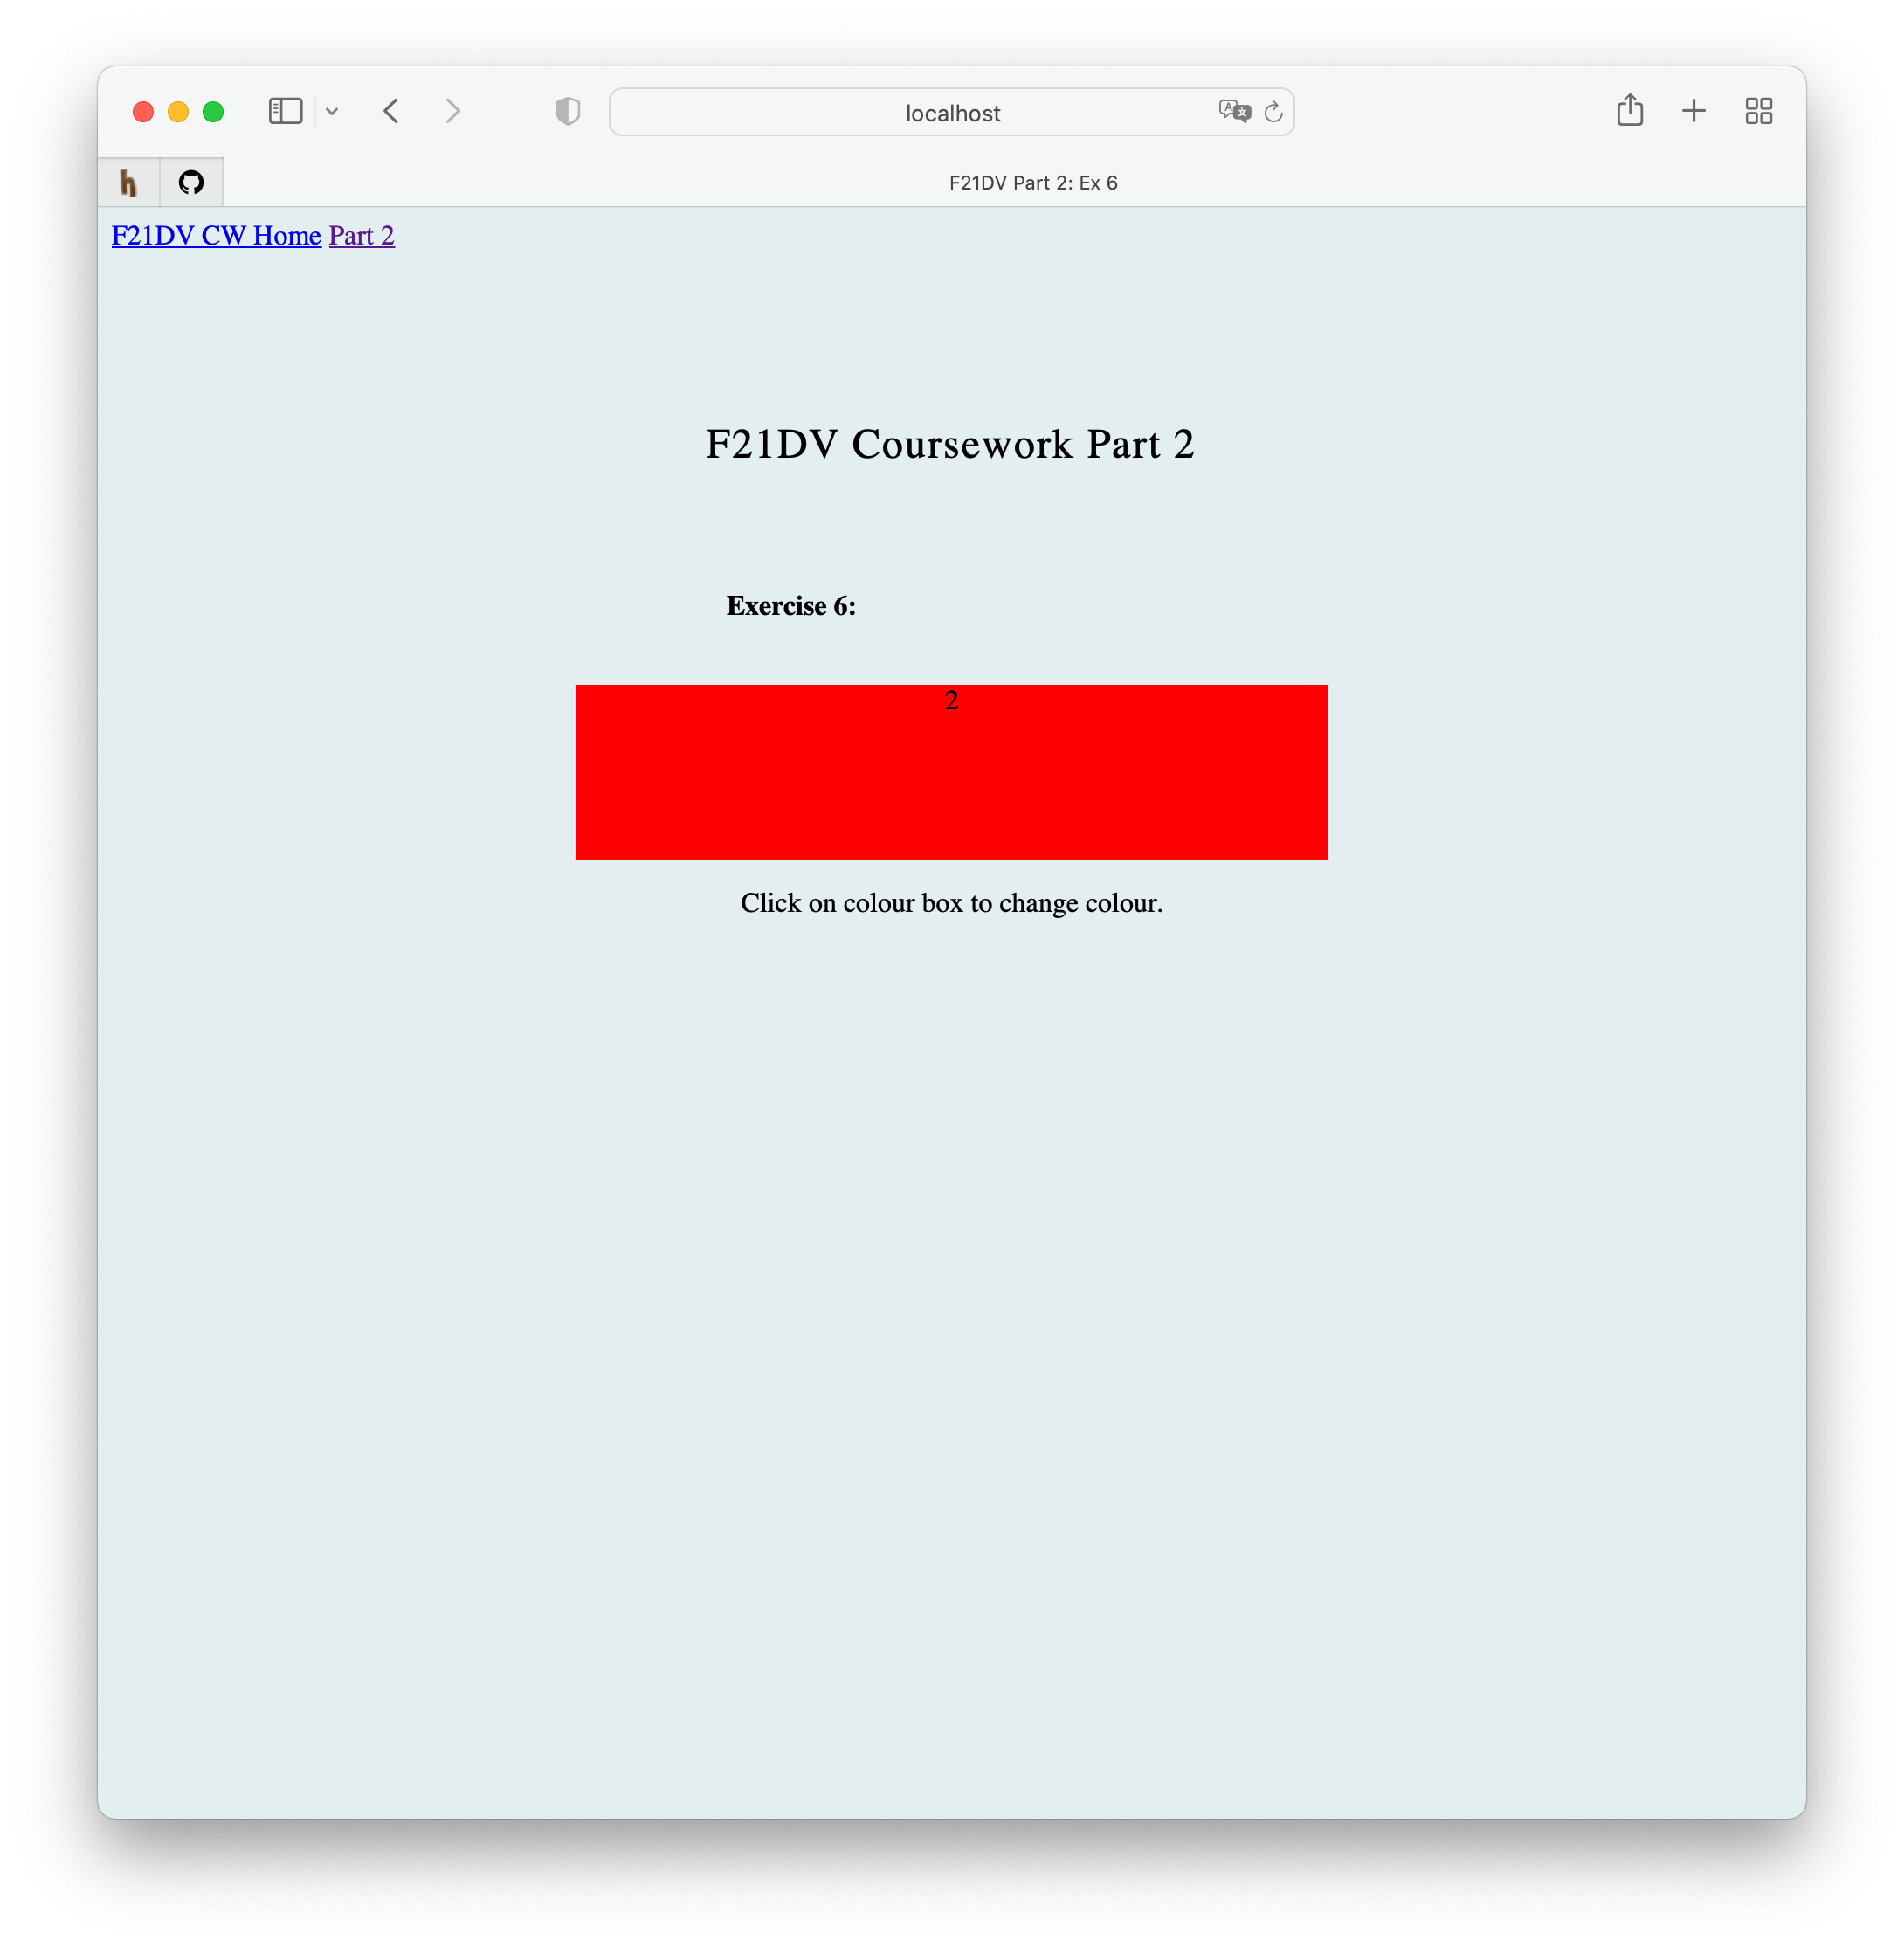
\includegraphics[width = 7.5cm]{images/ex6_2.png}
    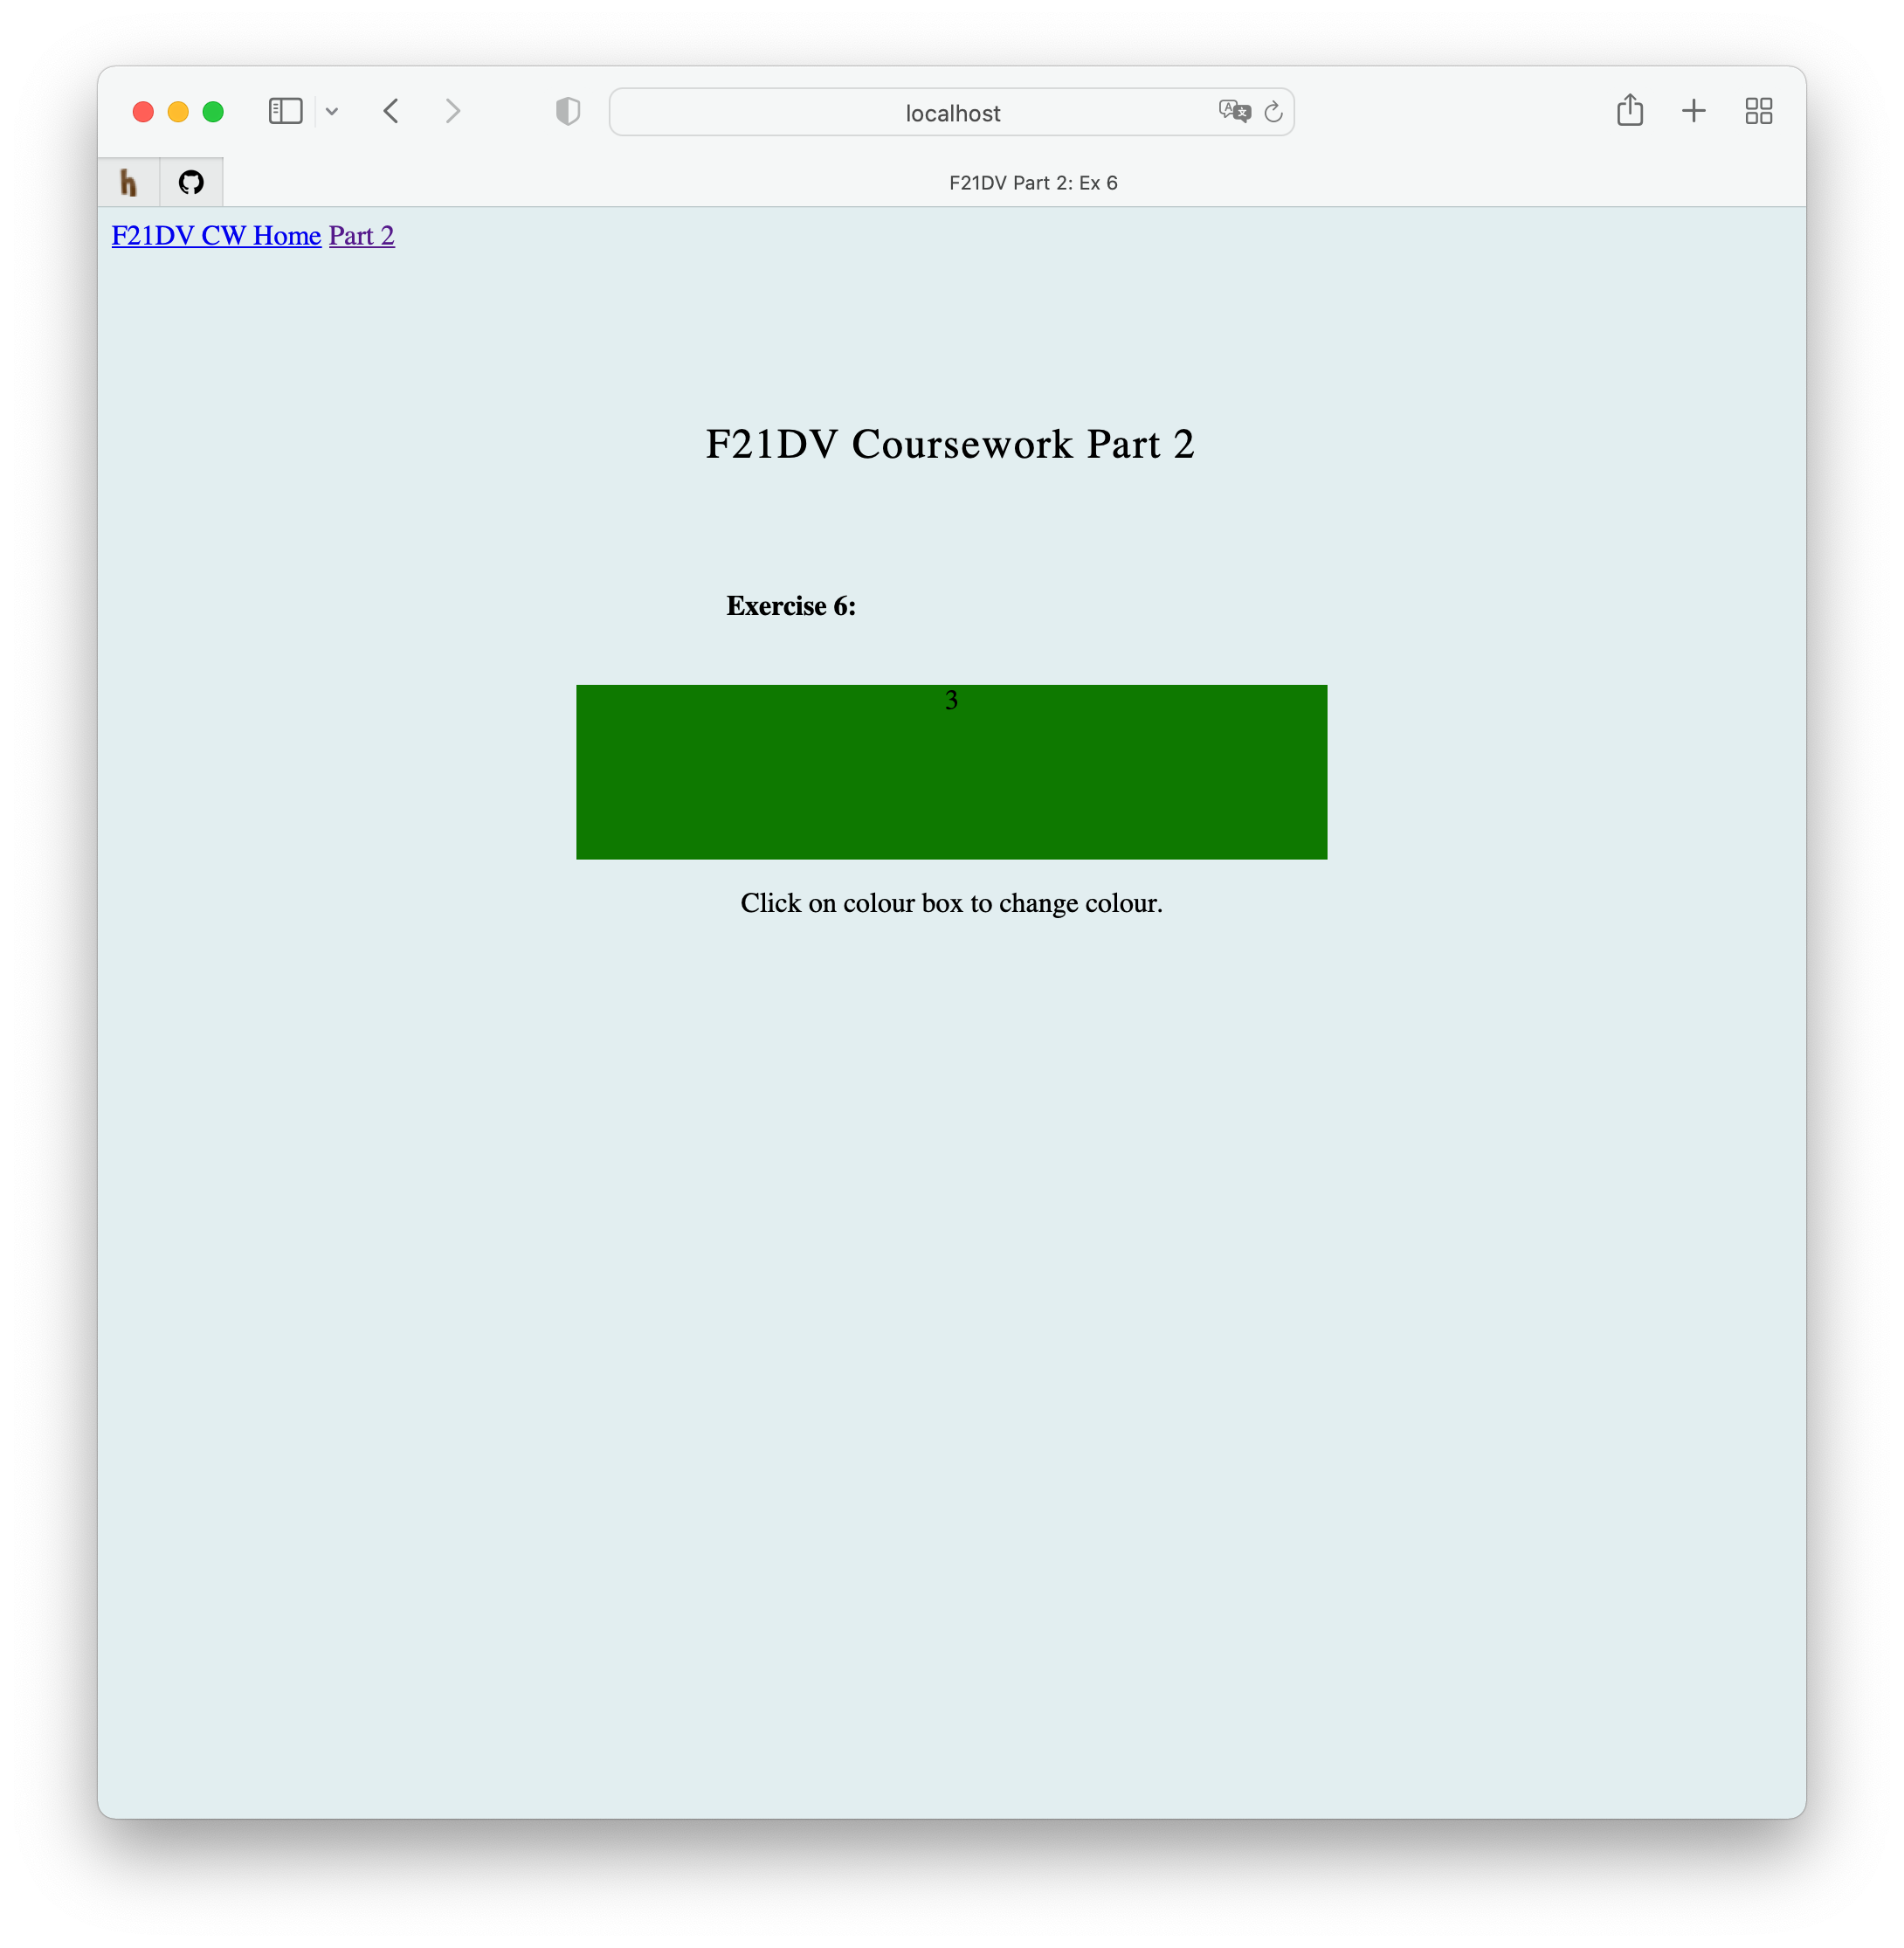
\includegraphics[width = 7.5cm]{images/ex6_3.png}
    \label{fig:ex6}
    \caption{Exercise 6}
\end{figure}
\FloatBarrier
\lstinputlisting[language=JavaScript]{../../public/js/part2/task6.js}
Figure \ref{fig:ex6} shows a coloured div with a number on it. On click, this div will transition to ``2'' and change to red, and then to ``3'' and then to green. Finally it will transition back to the original form. From listing above, we could see that this is done by using the transition upon mouse click, then changing the attributes of the div.

\end{document}